\documentclass{article}
\usepackage{setspace}
\usepackage{amsfonts}
\usepackage{graphicx}
\usepackage{amsmath}
\graphicspath{{./figures/}}
 
%----------------------------------------------------------------------------------------
%     AUTHORS and ABSTRACT
%----------------------------------------------------------------------------------------

\title{Plasma Modeling with the Heterogeneous Multiscale Method}
\author{Jeff Haack, Michael Murillo, Jacob Price, Gil Shohet}

\begin{document}
\maketitle

\begin{abstract}
Many phenomena can be described at different levels of detail by varying the choice of physical model. High-fidelity microscopic models generally come with an increased computational cost compared to low-fidelity macroscopic models. It is often the case that we desire the detail of the microscopic model on macroscopic scales. The heterogeneous multiscale method (HMM) provides a computational and analytical link between disparate physical models. It can be used to hybridize physical models in a way that improves the accuracy of the macroscale model while avoiding much of the computational expense of the microscale model. Accurately modeling plasmas generally requires expensive microscale models, so exploiting scale disparities has the potential to provide significant computational benefits. Given an accurate relaxation parameter, the Bhatnagar-Gross-Krook (BGK) approximation is an effective and efficient kinetic model for plasmas that are near equilibrium. This parameter, however, is difficult to know \emph{a priori}. Molecular dynamics offers a fully detailed model for ionic motion, but is computationally intensive. In this paper, we present a proof-of-principle of HMM as a modeling method for plasmas. Simulations using the hybrid kinetic-molecular dynamic model are both more accurate than the kinetic model alone, and orders of magnitude more efficient than the molecular dynamics model alone.
\end{abstract}

\pagebreak

%----------------------------------------------------------------------------------------
\section{Introduction}
%----------------------------------------------------------------------------------------

%----------------------------------------------------------------------------------------
\subsection{Multiscale modeling}
%----------------------------------------------------------------------------------------

Most mathematical and scientific problems contain phenomena with widely varying length and time scales of interest. Multiscale modeling aims to take advantage of this disparity to understand complex behavior at the desired level of detail \cite{weinan2011principles}. Multiphysics problems are a prototypical example of problems that are well-addressed by a multiscale approach. There is a hierarchy of physical models that allow systems to be modeled with varying degrees of detail, illustrated in Figure \ref{HMMhierarchy}. Quantum mechanics provides a complete description of physical interactions, but is often computationally and analytically intractable for all but the simplest systems. From quantum mechanics, one can derive laws of molecular dynamics (MD) as a more tractable, but less detailed physical description than the wavefunctions of quantum mechanics. These laws of motion are governed by interparticle potentials. From molecular dynamics, kinetic theory (KT) can be derived as a statistical description of molecular motion. Here, collisional cross-sections, an abstract quantity that averages away the behavior of individual particles, governs the evolution of the system. An even coarser model, hydrodynamics, can be derived either directly from molecular dynamics or from kinetic theory. Here, equations of state, which contain less detail than cross-sections, determine system behavior. With each step up the hierarchy, physical detail is generally sacrificed for greater computational efficiency.

\begin{figure}[h]
    \center 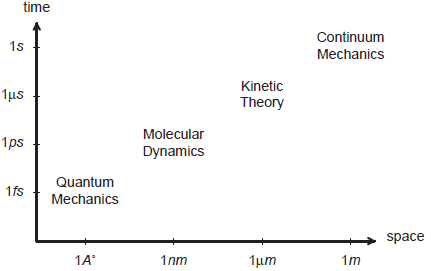
\includegraphics[width=0.7\linewidth]{hierarchy.png}
    \caption{Multiscale model hierarchy \protect\cite{weinan2007heterogeneous}. As we progress up the hierarchy, the sizes of the spatial and temporal domains we can compute reasonably with a model increase, but the level of detail decreases. HMM seeks to construct a hybrid method that joins two models at different levels in the hierarchy.}
	\label{HMMhierarchy}
\end{figure}

Unlike many multiscale models that use macroscale models to accelerate fully microscale simulations, the heterogeneous multiscale method (HMM) takes a top-down approach to multiphysics modeling \cite{weinan2007heterogeneous}. Multiple levels of detail are combined such that the models are mathematically consistent. HMM focuses on the coarsest (macroscale) model because it can be efficiently computed over much longer time scales than the more detailed (microscale) model. The goal is to minimize the computational time spent in the fine regime, using the microscale model only when it is critical to the accuracy of the solution. The two regimes are connected by a \emph{compression} operator, which compresses the necessary information in the microscale system into a consistent macroscopic description of the same system, and a \emph{reconstruction} operator, which generates a microscale system that matches the properties of the macroscale \cite{weinan2007heterogeneous}. The result is a hybrid simulation method that retains much of the computational speed of the coarse model with much of the accuracy of the fine model. This is essential when facing problems that have a large spatial or temporal region of interest, but which also include regions or aspects of interest that require microscopic detail. A full microscopic simulation would be prohibitively expensive, and a full macroscopic simulation would overlook crucial physical behavior in the domain. HMM is ideally suited to these types of problems.

Most HMM problems belong to one of two categories, which are outlined in Figure \ref{TypeABexamples}. \emph{Type A} problems use the microscale model in isolated regions, such as material defects, interfaces, or shocks, where the macroscale model is insufficient to model the system. \emph{Type B} problems exploit the microscale to provide an informed estimate of parameters that are necessary to close the macroscale system. A range of example applications of \emph{Type A} and \emph{Type B} problems is provided in \cite{weinan2007heterogeneous}. See \cite{ren2005heterogeneous} for detailed solutions of \emph{Type A} and \emph{Type B} problems using a combination of hydrodynamics and molecular dynamics. The problem we are solving is of \emph{Type B}; we use molecular dynamics simulations on the microscale to periodically provide an estimate of the relaxation parameter in our macroscale kinetic theory model. This general strategy is illustrated in Figure \ref{HMM}.
\begin{figure}[h]
    %\center 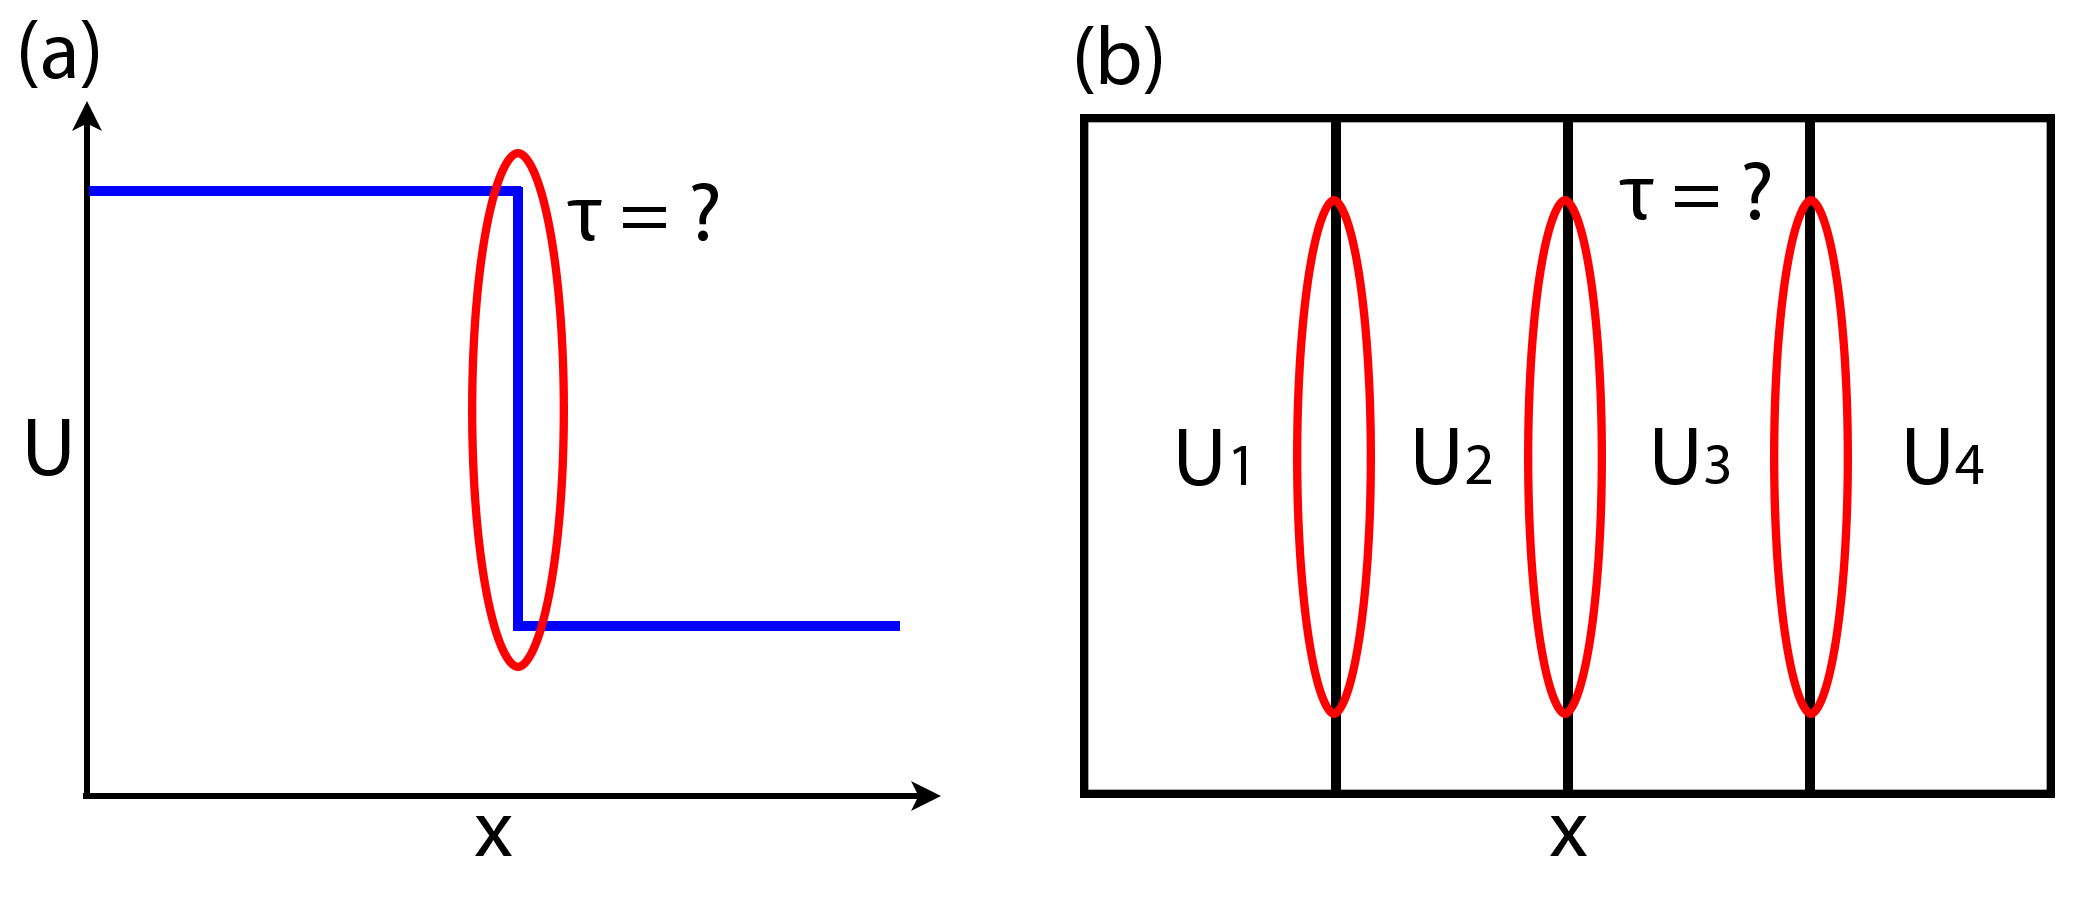
\includegraphics[width=0.8\linewidth]{typeABexample.jpg}
	\caption{Let $\tau$ be some quantity, such as the stress tensor, that is required to compute fluxes. (a): \emph{Type A} problem. There is an isolated discontinuity, for example a shock, in some quantity $U$. In the rest of the domain constitutive relations can be used to compute $\tau$, but in the discontinuity region, a microscale model is used since constitutive relations are insufficient. (b): \emph{Type B} problem. There is no sufficient constitutive model for $\tau$, so $\tau$ is computed at all cell interfaces using a constrained microscale model.}
	\label{TypeABexamples}
\end{figure}

\begin{figure}[ht]
	\center 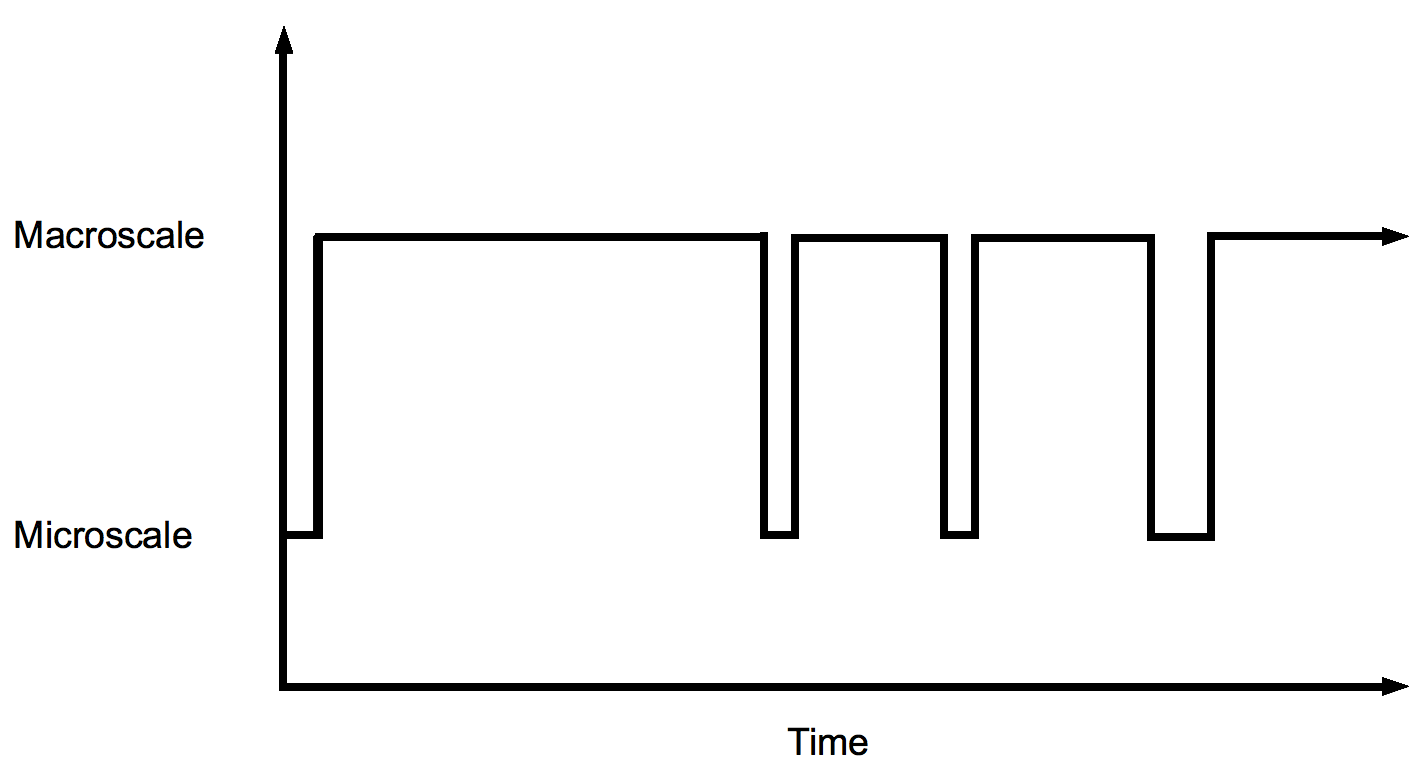
\includegraphics[width=.8\linewidth]{scheme.png}
	\caption{Illustration of the computational time spent in different computational regimes during an HMM simulation. In our system, the microscale is molecular dynamics simulation and the macroscale is kinetic theory simulation. Lines moving vertically upward correspond to the compression operator, lines moving vertically downward correspond to the reconstruction operator.}
	\label{HMM}
\end{figure}

%----------------------------------------------------------------------------------------
\subsection{Plasmas}
%----------------------------------------------------------------------------------------

Plasmas are electrically neutral systems of electrons and ions in which each ion interacts with many neighbors, making collective effects critical \cite{sturrock1994plasma}. Because opposite charges attract, each positive ion tends to be surrounded by a cloud of negatively charged background electrons which effectively ``screen'' the electrostatic field \cite{chen2006plasma}. The length scale of this near-neighbor interaction is represented by the \emph{Debye length} $\lambda$. This causes the potential around ions to fall rapidly, limiting the relevant interaction range between charged particles to a few Debye lengths. Examples of plasmas include astrophysical phenomena, such as stars and the interplanetary medium, terrestrial phenomena, such as lightning and aurorae, and technological constructs, such as plasma televisions and the materials used in fusion reactor research. Plasmas can exist at a wide range of temperatures and can exhibit a wide degree of coupling. We focus on plasmas that are moderately coupled, between the fully molecular and fully hydrodynamic regimes.

In this report we develop a hybrid multiphysics framework for modeling plasmas using the heterogeneous multiscale method (HMM). To model our system we combine the Bhatnagar-Gross-Krook (BGK) appoximation to the Boltzmann equation with molecular dynamics to model the time-evolution of a plasma system. This proof-of-principle model is designed to be mathematically rigorous and as general as possible. We develop the framework to model a class of problems involving weakly to moderately coupled plamas. We choose this regime because very weakly coupled plasmas can be better modeled as ideal gases and highly coupled plasmas can be better modeled using hydrodynamic relations. In the moderately-coupled regime, kinetic effects are significant. This formulation is novel in two ways: to our knowledge this is the first HMM formulation to combine molecular dynamics with kinetic theory, and also the first attempt to model plasmas using HMM. %This framework is then used to analyze several open questions in plasma modeling in the context of fusion reactors.

%----------------------------------------------------------------------------------------
\section{Model Formulation}
%----------------------------------------------------------------------------------------

Our model system is plasma simulated on a three-dimensional periodic domain, shown in Figure \ref{OVITO}. Periodic boundary conditions effectively approximate the behavior of a much larger domain, since ion interactions are screened by the background electrons. A screened potential avoids the additional complexity and computational cost of explicitly modeling electrons. This is a sufficient description of physical systems in which we are only interested in ion behavior and where the time scale of plasma interactions is much slower than the timescale of electron motion.
\begin{figure}[h]
   % 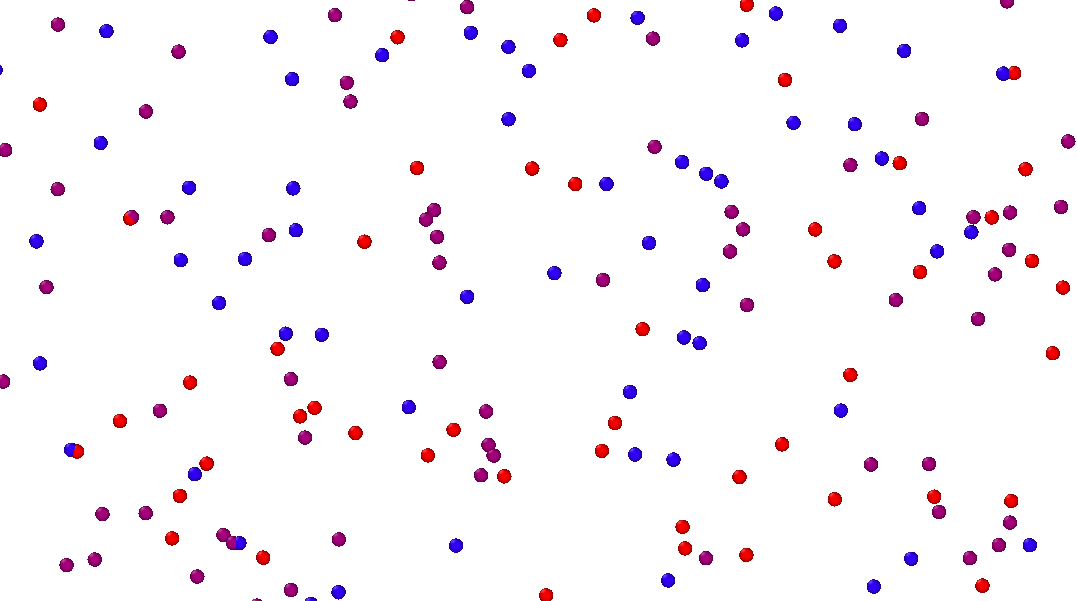
\includegraphics[width=0.8\linewidth]{OVITO.png}
	\caption{A cross-section of the three-dimensional periodic domain of simulation. Electrons are modeled implicitly through the screened potential. There may be multiple ion species, denoted by the different colors.}
	\label{OVITO}
\end{figure}

To use HMM to simulate this system, we select the Bhatnagar-Gross-Krook (BGK) approximation of the Boltzmann equation as our coarse (macroscale) kinetic theory model and molecular dynamics as our fine (microscale) model. An advantage of the BGK model is that the quantities we must derive from the molecular dynamics simulations, the relaxation times $\tau_{kl}$ for species $k$ toward its equilibrium with species $l$, are low-dimensional, local quantities, depending only on position. This is in contrast to the collisional cross-sections needed to connect MD to a Boltzmann kinetic formulation or the two-particle correlation functions $f_{kl}$ needed to connect MD to the BBGKY hierarchy, both of which are significantly more difficult to compute from MD. The quantity of interest in the BGK model is the distribution of each ion species. For ion species $k$, we represent this distribution by $f_k(\mathbf{r},\mathbf{v})$, which gives the particle density of species $k$ at position $\mathbf{r}=(x,y,z)$ with velocity $\mathbf{v}=(v_x,v_y,v_z)$. $f_k$ is normalized such that integrating $f_k$ over a region $A$ in phase space gives the expected number of particles in $A$ at time $t$. The partial differential equation governing this distribution is
\begin{equation}
\begin{split}
&\frac{\partial f_k}{\partial t}+\mathbf{v}\cdot\nabla_\mathbf{r}f_k-\frac{Z_ke}{m_k}\nabla_\mathbf{r}\phi(\mathbf{r},t)\cdot\nabla_\mathbf{v}f_k=\sum_l\frac{f_{kl}^{eq}-f_k}{\tau_{kl}}\\
&\left(\bigtriangleup_\mathbf{r}-\frac{1}{\lambda^2}\right)\phi(\mathbf{r},t)=-\frac{1}{\epsilon_0}\rho(\mathbf{r}',t)\\
&f_k(\mathbf{r},\mathbf{v},0)=f_{k}(\mathbf{r},\mathbf{v})\\
&\left.f_k(\mathbf{r},\mathbf{v},t)\right|_{x=0}=\left.f_{k}(\mathbf{r},\mathbf{v},t)\right|_{x=L_x},\;\;\;\;
\left.\phi(\mathbf{r},\mathbf{v},t)\right|_{x=0}=\left.\phi(\mathbf{r},\mathbf{v},t)\right|_{x=L_x}\\
&\left.f_k(\mathbf{r},\mathbf{v},t)\right|_{y=0}=\left.f_{k}(\mathbf{r},\mathbf{v},t)\right|_{y=L_y},\;\;\;\;
\left.\phi(\mathbf{r},\mathbf{v},t)\right|_{y=0}=\left.\phi(\mathbf{r},\mathbf{v},t)\right|_{y=L_y}\\
&\left.f_k(\mathbf{r},\mathbf{v},t)\right|_{z=0}=\left.f_{k}(\mathbf{r},\mathbf{v},t)\right|_{z=L_z},\;\;\;\;
\left.\phi(\mathbf{r},\mathbf{v},t)\right|_{z=0}=\left.\phi(\mathbf{r},\mathbf{v},t)\right|_{z=L_z}
\end{split}
\label{eq:BGK}
\end{equation}
Here, $Z_k$ is the charge of the ion and $m_k$ is its mass. $\phi(\mathbf{r})$ is the electric potential at position $\mathbf{r}$ due to all the ions of all species in the system. $e$ is the unit charge, $\epsilon_0$ is the vacuum permittivity, $\rho$ is the charge density due to every ion species, and $\lambda$ is the Debye length describing the degree of electron screening. $f_{kl}^{eq}$ is the equilibrium distribution of the mixture of ion species $k$ and $l$, and $\tau_{kl}$ is the time scale for relaxation towards this equilibrium distribution. $f_{kl}^{eq}$ is constructed such that the conservation laws are satisfied. $\tau_{kl}$ is the required input quantity from MD to the BGK model.

In the MD model, we have $N$ ions that are individually tracked according to the Hamiltonian equations
\begin{equation}
\begin{split}
\frac{\partial \mathbf{r}_i}{\partial t}&=\frac{1}{m_i}\nabla_{\mathbf{v}_i} H\\
\frac{\partial \mathbf{v}_i}{\partial t}&=-\frac{1}{m_i}\nabla_{\mathbf{r}_i}H\\
H(\{\mathbf{r}_k\}_{k=1}^N,\{\mathbf{v}_k\}_{k=1}^N)&=\sum_\alpha\left[\frac{m_\alpha|\mathbf{v}_\alpha|^2}{2}+\sum_{\alpha<j}U_{\alpha j}(\mathbf{r}_\alpha,\mathbf{r}_j)\right].
\end{split}\label{eq:MD}
\end{equation}
Here $\mathbf{r}_i$ and $\mathbf{v}_i$ are the position and velocity of ion $i$. $H$ is the Hamiltonian of the system. Ions evolve according to these simple equations in a periodic three-dimensional box. The potential energy $U_{ij}(\mathbf{r}_i,\mathbf{r}_j)$ represents the potential energy of particle $i$ due to particle $j$, screened by the electrons. It depends upon the identity of the two particles, as well as their positions. Let the indices of the particles that are of species one be expressed as $S_1=\{1,\dots, N_1\}$ where $N_1$ is the number of ions of species one. Similarly, the indices of species $k$ are $S_k=\{1+\sum_{l=1}^{k-1} N_l,\dots,\sum_{l=1}^kN_l\}$. Interparticle potentials can thus be written as $U_{ij}(\mathbf{r}_i,\mathbf{r}_j)=U_{\{kl\}}(\mathbf{r}_i,\mathbf{r}_j)$ where $i\in S_k$ and $j\in S_l$.  We leave this potential general when deriving the kinetic equations, such that this derivation is generalizable to any desired potential. 









 Let ions of species $k$ have mass $m_k$ and charge $Z_k$. Using the Yukawa potential to simulate electron screening, the potential energy between two ions at position $\mathbf{r}$ and $\mathbf{r}'$ with charges $Z_k$ and $Z_l$ respectively is
\begin{equation}U_{\{kl\}}(\mathbf{r},\mathbf{r}')=\frac{Z_kZ_le^2}{4\pi\epsilon_0}\frac{e^{-|\mathbf{r}-\mathbf{r}'|/\lambda}}{|\mathbf{r}-\mathbf{r}'|}.\label{eq:yukawa}
\end{equation}

BGK and MD models have a vast history of analytical and computational investigation. The HMM model requires us to connect them in a rigorous and explicit manner.





%----------------------------------------------------------------------------------------
\subsection{Multiscale derivation}
%----------------------------------------------------------------------------------------

HMM links disparate physical scales as closely as possible. Consequently, it is important to undergo a rigorous and detailed derivation of the manner in which the two scales are connected. This derivation can be seen in detail in the appendix, but it is summarized here.

The distribution of species $k$ is represented in MD as the expected value of the Klimontovich distribution $\mathcal{N}_k$:
\begin{equation}
\mathcal{N}_k(\mathbf{r},\mathbf{v},\{\mathbf{r}_\alpha\}_{\alpha=1}^{N},\{\mathbf{v}_\alpha\}_{\alpha=1}^{N},t)=\sum_{i\in S_k}\delta\left(\mathbf{r}-\mathbf{r}_i(t)\right)\delta\left(\mathbf{v}-\mathbf{v}_i(t)\right).
\end{equation}By taking the time derivative of the expected value of $\mathcal{N}_k$, and making the BGK approximation to the Boltzmann collision operator to separate the electrical and collisional components, it can be shown that
\[\frac{\partial f_k}{\partial t}+\mathbf{v}\cdot \nabla_\mathbf{r}f_k-\nabla_\mathbf{r}\sum_l\left(\int U_{\{kl\}}(\mathbf{r},\mathbf{r}')n_l(\mathbf{r}',t)\,d\mathbf{r}'\right)\cdot \nabla_\mathbf{v}f_k=\sum_l\frac{f_{kl}^{eq}-f_k}{\tau_{kl}}.
\]This is the governing BGK equation for a pairwise potential $U_{\{kl\}}$, and can be used to construct HMM simulations with a variety of potentials. Using the Yukawa potential (\ref{eq:yukawa}) for $U_{\{kl\}}$ yields the BGK equation we simulate (\ref{eq:BGK}).

The relaxation times, $\tau_{kl}$ remain undefined, and there is no standard formula through which to compute them. Instead, we select the $\tau_{kl}$ such that the rates of change of key physical quantities in the BGK model match observed rates in an MD simulation. First, the BGK equation possesses an H-theorem. That is, the negative entropy-like quantity 
\[\mathcal{H}(t) = \iint f(\mathbf{r},\mathbf{v},t)\log(f(\mathbf{r},\mathbf{v},t))\,d\mathbf{r}\,d\mathbf{v}.
\]The time derivative of $\mathcal{H}$ can be thought of as an ``entropy production rate.'' Observe also that the contributions of each species can be decomposed by defining
\begin{equation}
\mathcal{H}_k(t)=\iint f_k(\mathbf{r},\mathbf{v},t)\log(f(\mathbf{r},\mathbf{v},t))\,d\mathbf{r}\,d\mathbf{v}.
\end{equation}In order to spatially decompose the entropy production, we discretize the $\mathbf{r}$ integral according to the coarse grid:
\[\mathcal{H}(t)\approx\sum_k\sum_i (\Delta r)^d\int f_k(\mathbf{r}_i,\mathbf{v},t)\log(f(\mathbf{r}_i,\mathbf{v},t))\,d\mathbf{v}.
\] For simulations with multiple ionic species, we also consider the kinetic energy exchange between species. The kinetic energy of species $k$ at $\mathbf{r}$ is defined as
\begin{equation}K_k(\mathbf{r},t)=\int \frac{1}{2}m_k|\mathbf{v}|^2f_k(\mathbf{r},\mathbf{v},t)\,d\mathbf{v}.
\end{equation}
We can compute the rates of change of $\mathcal{H}$ and $K_k$ from a numerical simulation. By using the BGK equation (\ref{eq:BGK}), we can also express these rates in terms of the unknown $\tau_{kl}(\mathbf{r})$. By setting these rates equal, decomposing terms into contributions from separate species at each position $\mathbf{r}_i$, and solving for the $\tau_{kl}(\mathbf{r})$, we derive the following formulae for $\tau_{kl}$:
\begin{align}
\begin{split}
 \tau_{kk}(\mathbf{r}_i)=&\left(\int (f_{kk}^{eq}(\mathbf{r}_i,\mathbf{v})-f_k(\mathbf{r}_i,\mathbf{v},t))\log(f(\mathbf{r}_i,\mathbf{v},t)\right)\\&\bigg/\bigg(\frac{\partial \mathcal{G}_k^{MD}(\mathbf{r}_i,t)}{\partial t}+\int \mathbf{v}\cdot\nabla_\mathbf{r}[f(\mathbf{r}_i,\mathbf{v},t)](\log(f(\mathbf{r},\mathbf{v},t))+1)\,d\mathbf{v}\\&-\sum_{k\neq l}\frac{1}{\tau_{kl}(\mathbf{r}_i)}\int(f_{kl}^{eq}(\mathbf{r}_i,\mathbf{v})-f_k(\mathbf{r}_i,\mathbf{v},t))(\log(f(\mathbf{r}_i,\mathbf{v},t)))\,d\mathbf{v}\bigg),
\end{split}\label{eq:taukk}
\end{align}
where $\frac{\partial \mathcal{G}_k^{MD}}{\partial t}$ is the statistically observed value of
\begin{equation}
\mathcal{G}_k(\mathbf{r}_i,t)=(\Delta r)^d\int f_k(\mathbf{r}_i,\mathbf{v},t)\log(f(\mathbf{r}_i,\mathbf{v},t))\,d\mathbf{v}. 
\end{equation}Also,
\begin{align}
 \tau_{kl}(\mathbf{r})=&\left(K_{kl}^{eq}(\mathbf{r})-K_k(\mathbf{r},t)\right)\bigg/\left(\frac{\partial K_{kl}^{MD}(\mathbf{r},t)}{\partial t}-Z_k e \mathbf{E}_l(\mathbf{r})\cdot n_k(\mathbf{r})\mathbf{u}_k(\mathbf{r})\right),\label{eq:taukl}
\end{align}
where $K_{kl}^{eq}$ is the kinetic energy density of the equilibrium distribution, $\mathbf{E}_l$ is the electric field at $\mathbf{r}$ due to species $l$, $n_k$ is the ion density of species $k$ at $\mathbf{r}$, and $u_k$ is the bulk velocity of species $k$ at $\mathbf{r}$.

We compute the statistical quantities at each position $\mathbf{r}$ $\mathcal{G}_k^{MD}$ and $K_{kl}^{MD}$ from MD simulations. The macroscale variables provide the boundary and initial conditions. The cells are initialized according to the macroscale distributions $f_k$. However, these distribution contains no knowledge of the particle correlations, complicating the task of placing particles in the MD domain. Naive particle placement necessarily leads to temperature changes in the initial steps of the MD simulation due to particles placed too near or far from one another, driving the distribution away from the desired initialization \cite{gericke2003disorder}. Given the microcell size, we place the correct number of particles of each type to satisfy the computed density. We initialize them using the Halton sequence, which yields a more correlated distribution than pseudorandom selections, allowing faster equilibration. We then run an equilibration phase, driving the system toward the correct $T_k$ with Langevin dynamics and periodic boundary conditions. and are periodically extended across the whole domain. Once equilibrated, we discard the velocities of each particle, and draw new velocities for every particle from the macroscale velocity distribution. Because this distribution is very discrete in the kinetic formulation, we linearly interpolate it before sampling. This method is able to accurately capture in MD at least the first four moments of the $f_k$ distribution with sufficient particles. Once this is done, the particles have correlated spatially and are distributed according to the correct velocity distribution. This is considered the ``initial condition'' for an MD simulation.

We then turn off the thermostat and allow the system to evolve with periodic boundary conditions. The data from the particle trajectories are used to compute the necessary statistical quantities. Because the $\tau_{kl}$ are local and the equilibration dynamics operate much faster than bulk motion, this simulations are perfectly tailored to provide the exact missing data needed for a macroscale timestep.

$\mathcal{G}_k^{MD}$ can be computed from its definition by approximating $f_k$ as a velocity histogram for the purposes of integration. The time derivative is computed with a simple centered difference formula. The rate of kinetic energy conversion between species is computed by explicitly computing the total kinetic energy of each species and computing explicitly how the force interactions with each other species alter this during each time step. These quantities ought to be ensemble averages, and so are both averaged over a period of time to approximate this.

In this way, the data from a brief MD simulation can be used to compute relaxation times such that the entropy production rates and energy exchange rates of the BGK simulation will match those observed in the MD simulation. With the compression and reconstruction operators fully defined, we may now use the HMM method to analyze a plasma system that requires large spatial or temporal scales, but microscopic detail.



%After the BGK simulation runs for a period of time, the distributions $f_k$ will have changed, and with them the relaxation times. Thus, it eventually becomes necessary to run a new MD simulation to update these parameters. We need a reconstruction operator to initialize an MD simulation given the distribution $f_k$.
%
%Suppose at time $t$, we have a distribution $f_k(x,\mathbf{v},t)$ from the kinetic simulation. At this time, we wish to update $\tau_{kl}$, and so must sample this distribution to place ions in the two-dimensional MD domain. However, this distribution contains no knowledge of the particle correlations, complicating the task of placing particles in the MD domain. Naive particle placement necessarily leads to temperature changes in the initial steps of the MD simulation due to particles placed too near or far from one another, driving the distribution away from the desired initialization \cite{gericke2003disorder}.
%
%We begin by initializing the MD distribution \emph{near} the distribution $f_k$. To do this, we compute the spatially dependent density $n_k(x)$ and temperature $T_k(x)$. Dividing the MD domain into the same number of cells as $x$ has grid points in the kinetic simulation, we place particles in each cell to match the density in that cell. We initialize them using the Halton sequence, which yields a more correlated distribution than pseudorandom selections, allowing faster equilibration. We then run an equilibration phase, driving each cell toward the correct $T_k(x)$ with Langevin dynamics. At the right and left side of each cell, we enforce reflective boundary conditions, such that each ion must stay within the cell in which it was originally placed. The particles \emph{do}, however, electrostatically interact with the ions in other cells. This model configuration is shown in Figure \ref{MDequil}. The result is that the particles in each cell are correlated consistently with the prescribed density and temperature. The inter-cell interactions should smooth the coarse distribution into something consistent on the fine scale.
%\begin{figure}[h]
%   \center 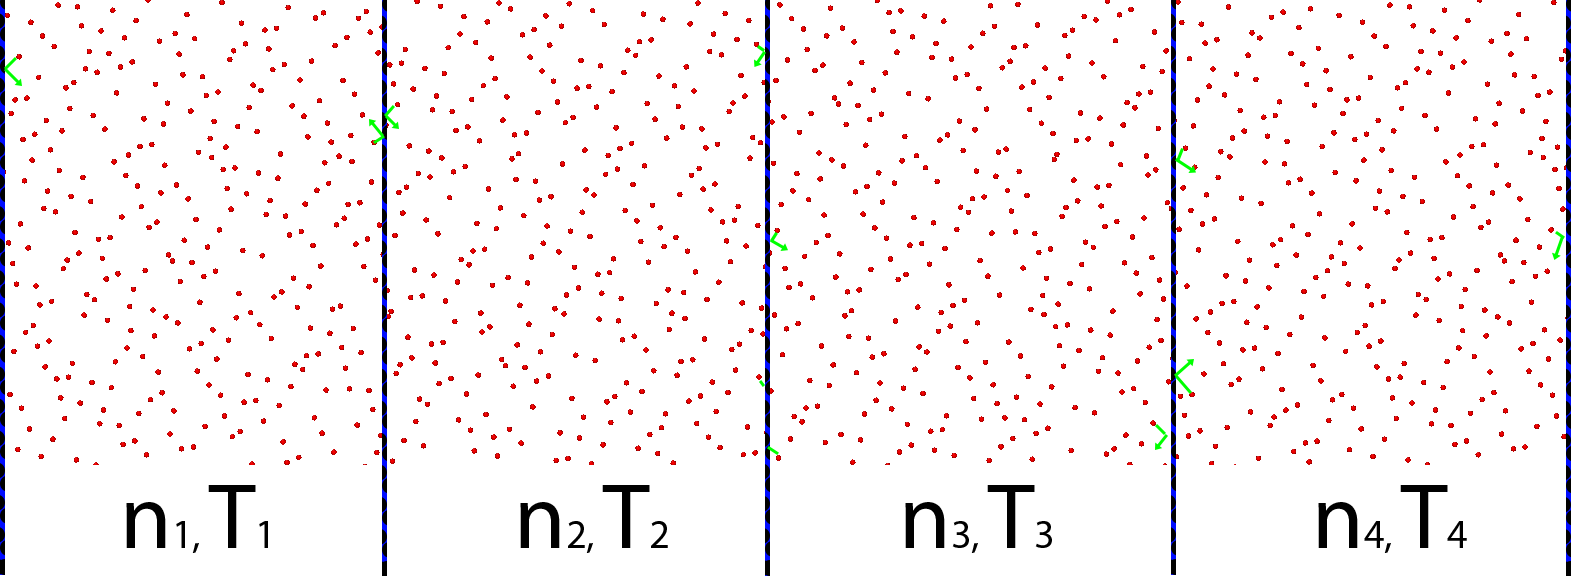
\includegraphics[width=0.8\linewidth]{equilibration.png}
%	\caption{Configuration of MD simulation during equilibration phase.}
%	\label{MDequil}
%\end{figure}

%Once equilibrated, we throw away the velocities of each particle, and draw new velocities for every particle in cell $x_i$ from the velocity distribution at $x_i$, $f_k(x_i,\mathbf{v},t)$. Because this distribution is very discrete in the kinetic formulation, we linearly interpolate it before sampling. This method is able to accurately capture in MD at least the first four moments of the $f_k$ distribution with sufficient particles. Once this is done, the particles have correlated spatially and are distributed according to the correct velocity distribution. This is considered the ``initial condition'' for an MD simulation.

%With the compression and reconstruction operators fully defined, we may now use the HMM method to analyze a plasma system that requires large spatial or temporal scales, but microscopic detail.

%----------------------------------------------------------------------------------------
\section{Method Verification}
%----------------------------------------------------------------------------------------

We have the theoretical basis for linking the MD and BGK models into a consistent HMM solver, but the programmatic link between the two was incomplete at the time of writing. To provide an initial comparison, both moels were used to solve an identical interface problem. In this problem of interest, a single ion species was initialized in an isothermal domain, with zero bulk velocity, such that the center region has a density three times that of the outer region. The simulation was then allowed to evolve for a time of $120\omega_0^{-1}$. The simulation was stopped at this end time due to time constraints on the MD. In the 1D-2V BGK solver, the spatial domain was discretized into 32 cells. The model was then evolved assuming a screened Poisson equation for the electric field, and using a naive first-order estimate of the relaxation timescale, $\tau = \omega_0^{-1}$. The hydrodynamic moments in the corresponding spatial regions were tracked throughout the 2D-2V MD simulation, which used 32,000 particles, to facilitate comparison. The conditions at the beginning and end of the simulation are shown in Figures \ref{Results0} and \ref{ResultsEnd} with axes labeled in the nondimensional units.

From Figure \ref{ResultsEnd}, we observe that the MD and BGK simulations yield qualitatively and even quantitatively similar results, even with a very naively calculated $\tau$. The noise that appears in the MD result is present mainly due to the small number of particles in each cell used to compute moments and the fact that time-averaging was not performed. In practice, a moving time averaging window would smooth the MD hydrodynamic moments. At the end time, the high density region in the BGK has expanded further than the high density region in the MD, suggesting the timescale associated with the BGK model is slightly faster than that for the MD in these conditions. This demonstrates the advantages we will gain when the HMM implementation allows us to inform $\tau$ through MD. The screened Poisson equation is not valid in 2D and only useful as a first-order approximation. This may also have played a role in the discrepancy. 

The BGK simulation completed in under a minute, compared with over 24 hours for the MD simulation. The large speedup gained from the BGK model compared with MD, combined with the close results even with a first-order approximation to $\tau$, suggests that very good results might be obtained with a better estimate of the collisional relaxation timescale using the method outlined above. We are optimistic that this implementation will provide stark benefits to plasma modeling in the near future.
\begin{figure}[h]
   % 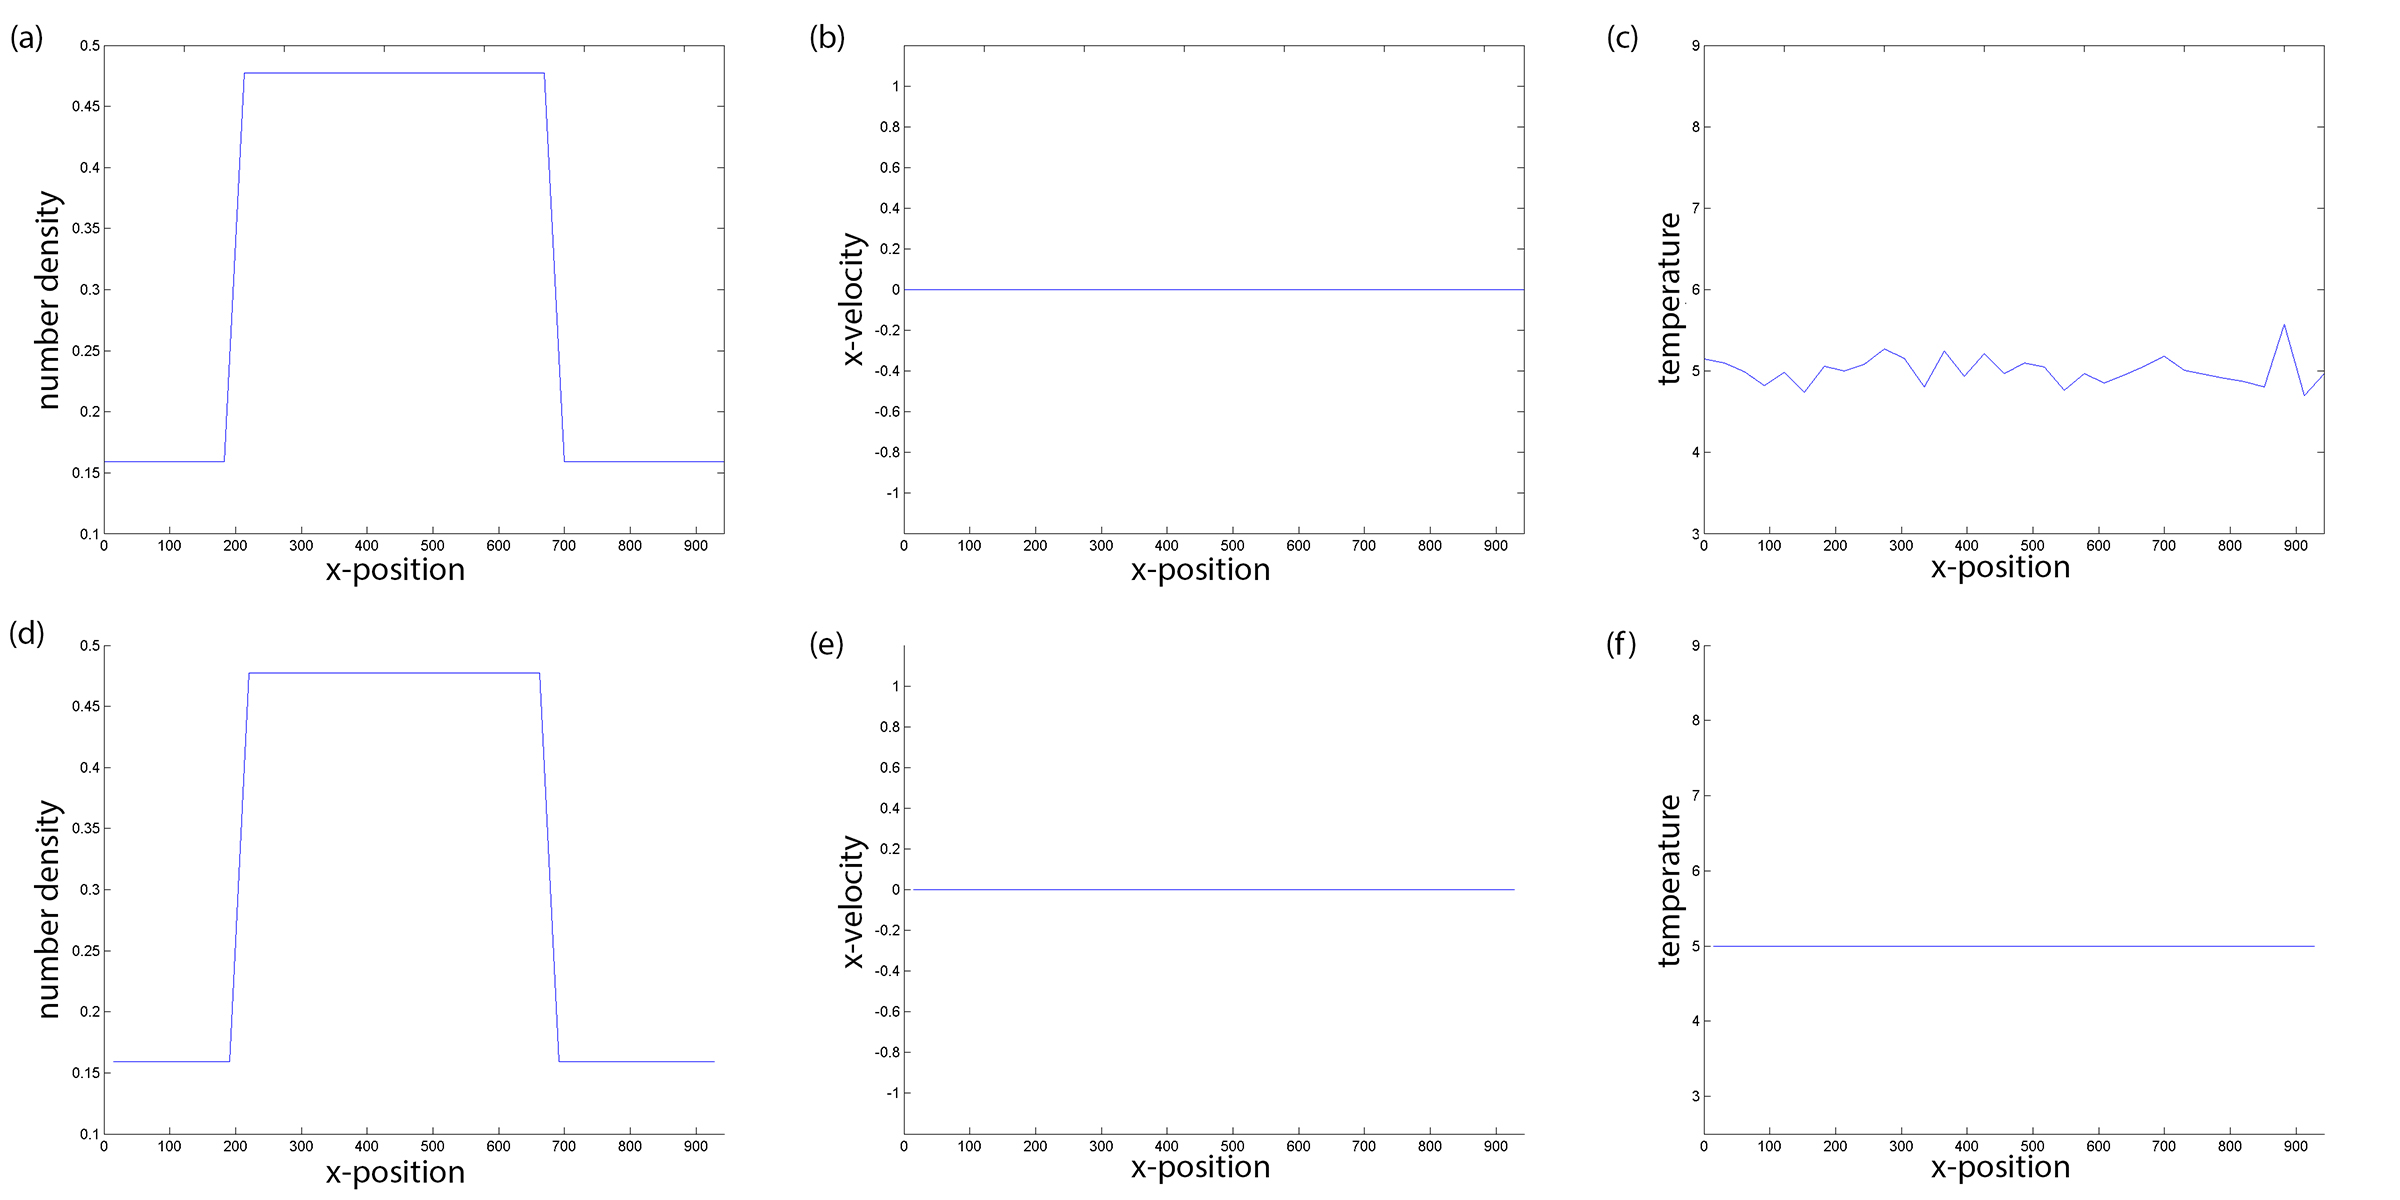
\includegraphics[width=\linewidth]{ResultsFrame0.jpg}
	\caption{Initial conditions for the MD (top) and BGK (bottom) simulations. (a)-(c): zeroth through second moments computed from MD. (d)-(f): zeroth through second moments computed from BGK.}
	\label{Results0}
\end{figure}
\begin{figure}[h]
   % 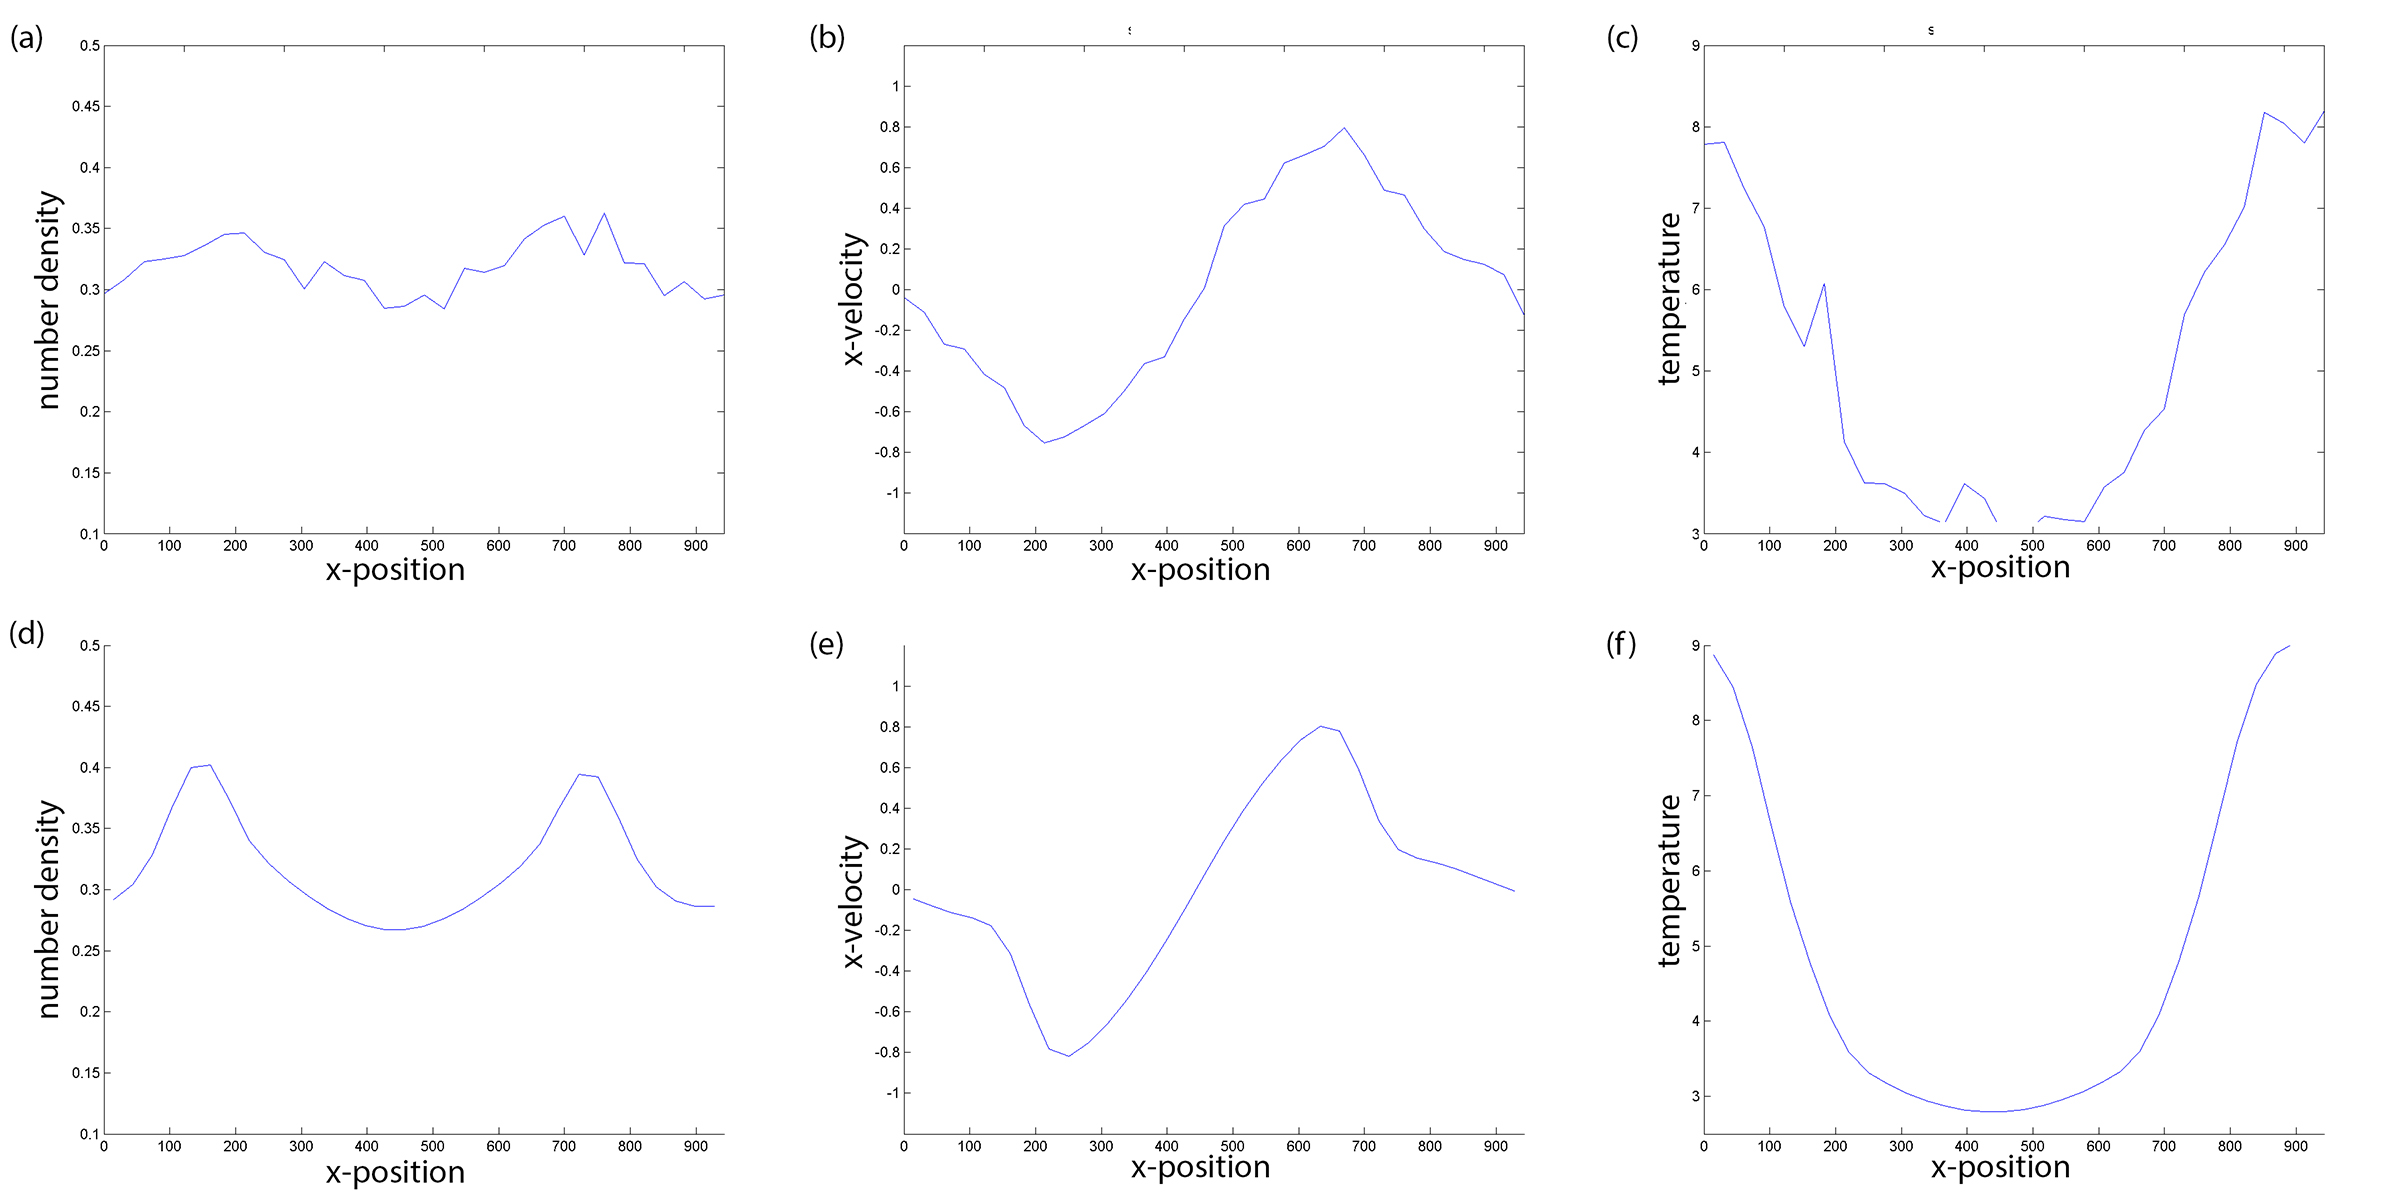
\includegraphics[width=\linewidth]{ResultsFrame401.jpg}
	\caption{State at $t=120\omega_0^{-1}$ for the MD (top) and BGK (bottom) simulations. (a)-(c): zeroth through second moments computed from MD. (d)-(f): zeroth through second moments computed from BGK.}
	\label{ResultsEnd}
\end{figure}

%----------------------------------------------------------------------------------------
%\section{Case Study 2: Fusion}
%----------------------------------------------------------------------------------------


%----------------------------------------------------------------------------------------
\section{Conclusions}
%----------------------------------------------------------------------------------------

The heterogeneous multiscale method is an exceptionally powerful tool for solving problems that contain multiple physical regimes. HMM provides a rigorous, well-defined means to build hybrid models that combine the accuracy of a fine-grained model with the computational efficiency of a coarse-grained model. This allows detailed and efficient exploration of multiscale phenomena. These phenomena include mesoscale systems that concurrently display macroscopic and microscopic behavior and systems with defects such as cracks or shocks.

In this report, we have demonstrated its power in simulating plasma using kinetic theory and molecular dynamics. Both models, given the same initial condition, evolve in nearly identical manners. Only the time scale of the kinetic model is incorrect. Once the models are coupled through $\tau_{kl}$, the kinetic model will accurately capture the behavior of the full microscale model with a computational speedup factor of hundreds to thousands, depending on the problem.

This proof-of-principle paves the way for additional improvements in the method. First of all, the method is currently implemented in Matlab. Converting this to another language would increase the efficiency even further and allow three-dimensional simulations. Second, our method is eminently paralellizable. The $\tau_{kl}$ are computed as ensemble averages. The accuracy of this could be improved by running many MD simulations in parallel, greatly decreasing statistical noise by making use of the Law of Large Numbers. One can also foresee running MD simulations and BGK simulations concurrently, updating $\tau_{kl}$ continuously, rather than periodically. The potential for additional speedups is significant and enticing.

Furthermore, in this report we have created a fully consistent multiscale connection between molecular dynamics and kinetic theory. This methodology can be adapted with no change to the formulation to study systems with different potentials, systems that incorporate electron motion, and systems of three dimensions. It allows for $n$ species with different charges and masses, and even interparticle potentials that differ more significantly than simply being scaled by the charge. Finally, we can modify our assumptions to connect MD to other kinetic models. For example, if we do not approximate $f_{kl}$, but instead compute it from MD, we can couple MD to the BBGKY hierarchy. We could also compute collisional cross-sections in order to couple MD with the Boltzmann equation.

These results are significant, as to our knowledge there does not exist an HMM model that couples molecular dynamics and kinetic theory. Our derivation here allows the coupling of MD to any number of kinetic theory formulations. Additionally, HMM has not, to our knowledge, been used to model plasmas. It is the opinion of the authors that HMM represents an important part of the future of computational physics. The applications include plasma modeling, mesoscale modeling, mathematical biology, high-accuracy hydrodynamic models, and countless more. This report is a definitive proof-of-principle of the applicability of HMM to plasma modeling, and further demonstrates the viability of HMM as a computational tool.

%----------------------------------------------------------------------------------------
\section{Acknowledgments}
%----------------------------------------------------------------------------------------

We would like to thank our mentors, Michael Murillo and Jeff Haack, for working with us on this project. Their project proposal was fascinating, and our many fantastic conversations with them led to countless breakthroughs. We also express our thanks to Jeff Haack and Mathieu Marciante, who provided the base codes for BGK and MD, respectively. Without these to build upon, we would have been unable to fully explore HMM in our brief time here. Thanks is also due to the Namb\'e group, which graciously allowed us to attend their quarterly meeting and present our results to plasma physicists from around the world.

Finally, we would like to thank the other students, administration, and lecturers of the Computational Physics Student Summer Workshop. Together, they gave us an enlightening, enriching, and enjoyable summer of research, and we hope we have established lasting relationships with the lab and our student colleagues.

\newpage
\appendix


\section{Mathematical details}



Our system is described in full detail when we evolve every ion in the molecular dynamics simulation according to the Hamiltonian equations (\ref{eq:MD}). We derive, from this starting point, the BGK kinetic theory formulation of the problem (\ref{eq:BGK}). We begin by constructing a Klimontovich distribution \cite{klimontovich1983kinetic} $\mathcal{N}_k$ for each species $k$ that stores the location $\mathbf{r}_i$ and velocity $\mathbf{v}_i$ of every ion of that species at a given time $t$:
\begin{equation}\mathcal{N}_k(\mathbf{r},\mathbf{v},\{\mathbf{r}_\alpha\}_{\alpha=1}^{N},\{\mathbf{v}_\alpha\}_{\alpha=1}^{N},t)=\sum_{i\in S_k}\delta\left(\mathbf{r}-\mathbf{r}_i(t)\right)\delta\left(\mathbf{v}-\mathbf{v}_i(t)\right)
\end{equation}where $\delta(x)$ is the Dirac delta function. Consider taking the time derivative of this distribution:

%We are interested in the time evolution of the Klimontovich distribution. Thus, an aside relating to distributions and their derivatives is warranted.

%----------------------------------------------------------------------------------------
%\subsection{Distributional derivatives}
%----------------------------------------------------------------------------------------

%Consider the set of test functions, $D(\mathbb{R})$ that are infinitely differentiable and have compact support. A distribution is a linear mapping $T: D(\mathbb{R})\to\mathbb{R}$. By convention, the operation of a distribution $T$ on a target function $f$ is written $\langle T,f\rangle$, and is defined as the integral over $\mathbb{R}$ of the product between $T(x)$ and $f(x)$. The Dirac delta ``function'' can thus be written $\langle \delta,f\rangle=f(0)$.

%The derivative of a distribution is defined as $\langle T',f\rangle=-\langle T,f'\rangle$. This is a consequence of integration by parts:
%\begin{eqnarray*}
%\langle T',f\rangle=\int_{-\infty}^\infty \delta'(x)f(x)\;dx=\left[f(x)\delta(x)\right]_{-\infty}^\infty-\int_{-\infty}^\infty \delta(x)f'(x)\;dx=-\langle T,f'\rangle.
%\end{eqnarray*}

%We discount the first term in the integration by parts because our test functions are considered equal to zero outside of a bounded set. Though we will not explicitly compute the derivative of $\delta(x)$, it suffices to show that it exists and is well-defined. The above definition of the distributional derivative also allows for a seamless use of the product and chain rules in their standard forms in the presence of distributions.  Our problem utilizes two-dimensional Dirac delta functions, defined as
%\[\delta(\mathbf{r})=\delta(r_x)\delta(r_y).
%\]The gradient of this function similarly exists:
%\begin{eqnarray*}
%\langle\nabla_\mathbf{r}\delta(\mathbf{r}),f\rangle=-\langle\delta(\mathbf{r}),\nabla_\mathbf{r}f\rangle.
%\end{eqnarray*}Gradients of two-dimensional delta functions are thus well defined.

\begin{align*}
\frac{\partial \mathcal{N}_k}{\partial t}=\sum_{i\in S_k}& \frac{\partial}{\partial t}\left[\delta(\mathbf{r}-\mathbf{r}_i(t))\delta(\mathbf{v}-\mathbf{v}_i(t))\right]\\
=\sum_{i\in S_k}& \delta(\mathbf{v}-\mathbf{v}_i(t))\frac{\partial}{\partial t}\delta(\mathbf{r}-\mathbf{r}_i(t))+\delta(\mathbf{r}-\mathbf{r}_i(t))\frac{\partial }{\partial t}\delta(\mathbf{v}-\mathbf{v}_i(t))\\
=\sum_{i\in S_k}&\bigg\{\delta(\mathbf{v}-\mathbf{v}_i(t))\frac{\partial(\mathbf{r}-\mathbf{r}_i(t))}{\partial t}\cdot\nabla_{(\mathbf{r}-\mathbf{r}_i)}[\delta(\mathbf{r}-\mathbf{r}_i(t))]\\
&+\delta(\mathbf{r}-\mathbf{r}_i(t))\frac{\partial(\mathbf{v}-\mathbf{v}_i(t))}{\partial t}\cdot\nabla_{(\mathbf{v}-\mathbf{v}_i)}[\delta(\mathbf{v}-\mathbf{v}_i(t))]\bigg\}\\
=\sum_{i\in S_k}&\bigg\{-\frac{\partial \mathbf{r}_i(t)}{\partial t}\delta(\mathbf{v}-\mathbf{v}_i(t))\cdot \nabla_\mathbf{r}[\delta(\mathbf{r}-\mathbf{r}_i(t))]\\&-\frac{\partial \mathbf{v}_i(t)}{\partial t}\delta(\mathbf{r}-\mathbf{r}_i(t))\cdot \nabla_\mathbf{v}[\delta(\mathbf{v}-\mathbf{v}_i(t))]\bigg\}.
\end{align*}

We now use the definition of the Hamiltonian. We focus our attention on particle $i$:
\begin{equation}
\frac{\partial \mathbf{r}_i}{\partial t}=\frac{1}{m_i}\nabla_{\mathbf{v}_i}H=\frac{1}{m_i}\nabla_{\mathbf{v}_i}\left(\sum_\alpha\left[\frac{m_\alpha|\mathbf{v}_\alpha|^2}{2}+\sum_{\alpha<j}U_{\alpha j}(\mathbf{r}_\alpha,\mathbf{r}_j)\right]\right)=\mathbf{v}_i.\label{dridt}
\end{equation}
We must require that the potential satisfy the constraint that $\sum_i\sum_{i<j}U_{ij}(\mathbf{r}_i,\mathbf{r}_j)$ be fixed under a permutation of particle indices. That is,
\[\sum_i\sum_{i<j} U_{ij}(\mathbf{r}_i,\mathbf{r}_j)=\sum_{p(i)}\sum_{p(i)<p(j)}U_{p(i),p(j)}(\mathbf{r}_{p(i)},\mathbf{r}_{p(j)})
\] for all permutations $\{1,2,\dots\}\to\{p(1),p(2),\dots\}$. This simply implies that the total potential energy is independent of the choice of indices, which is a natural requirement. Using this assumption, we permute the indices such that particle $i$ and particle $1$ switch places. That is, $p(i)=1$. Furthermore, let particle $i$ be a member of species $k$, so
\begin{align}
\begin{split}
\frac{\partial \mathbf{v}_i}{\partial t}=-\frac{1}{m_i}\nabla_{\mathbf{r}_i}H=&-\frac{1}{m_i}\nabla_{\mathbf{r}_i}\left(\sum_\alpha\left[\frac{m_\alpha|\mathbf{v}_\alpha|^2}{2}+\sum_{\alpha<j}U_{\alpha j}(\mathbf{r}_\alpha,\mathbf{r}_j)\right]\right)
\\=&-\frac{1}{m_i}\nabla_{\mathbf{r}_{p(i)}} \left[\sum_{p(\alpha)}\sum_{p(\alpha)<p(j)}U_{\alpha j}(\mathbf{r}_\alpha,\mathbf{r}_j)\right]\\
=&-\frac{1}{m_i}\nabla_{\mathbf{r}_{p(i)}}\left[\sum_{p(j)\neq 1}U_{ij}(\mathbf{r}_{p(i)},\mathbf{r}_{p(j)})\right]\\
=&-\frac{1}{m_i}\nabla_{\mathbf{r}_{p(i)}}\left[\sum_l\sum_{p(j)\in S_l,p(j)\neq 1}U_{\{kl\}}(\mathbf{r}_{p(i)},\mathbf{r}_{p(j)})\right].\label{dpidt}
\end{split}\end{align}
Abusing notation, let us redefine the indices such that $i=p(i)$. Using (\ref{dridt}) and (\ref{dpidt}), we find
\begin{align*}
\frac{\partial \mathcal{N}_k}{\partial t}=&\sum_{i\in S_k}\left[-\frac{\partial \mathbf{r}_i(t)}{\partial t}\delta(\mathbf{v}-\mathbf{v}_i(t))\cdot \nabla_\mathbf{r}\delta(\mathbf{r}-\mathbf{r}_i)-\frac{\partial \mathbf{v}_i(t)}{\partial t}\delta(\mathbf{r}-\mathbf{r}_i(t))\cdot \nabla_\mathbf{v}[\delta(\mathbf{v}-\mathbf{v}_i(t))]\right]\\
=&\sum_{i\in S_k}\bigg[-\mathbf{v}_i\delta(\mathbf{v}-\mathbf{v}_i(t))\cdot\nabla_\mathbf{r}\delta(\mathbf{r}-\mathbf{r}_i(t))\\&+\frac{1}{m_i}\delta(\mathbf{r}-\mathbf{r}_i(t))\nabla_{\mathbf{r}_i}\left[\sum_l\sum_{j\in S_l,j\neq 1}U_{\{kl\}}(\mathbf{r}_{i},\mathbf{r}_{j})\right]\cdot \nabla_\mathbf{v}\delta(\mathbf{v}-\mathbf{v}_i(t))\bigg]\\
=&\sum_{i\in S_k}\bigg[-\mathbf{v}_i\delta(\mathbf{v}-\mathbf{v}_i(t))\cdot\nabla_\mathbf{r}\delta(r-\mathbf{r}_i(t))\\&+\frac{1}{m_k}\delta(\mathbf{r}-\mathbf{r}_i(t))\nabla_{\mathbf{r}_{i}}\left[\sum_l\sum_{j\in S_l,j\neq 1}U_{\{kl\}}(\mathbf{r}_{i},\mathbf{r}_{j})\right]\cdot \nabla_\mathbf{v}\delta(\mathbf{v}-\mathbf{v}_i(t))\bigg].
\end{align*}

Using the identity $\mathbf{q}_i\delta(\mathbf{q}-\mathbf{q}_i)=-\mathbf{q}\delta(\mathbf{q}-\mathbf{q}_i)$, we can show
\begin{align*}
\frac{\partial \mathcal{N}_k}{\partial t}=&\sum_{i\in S_k}\bigg[-\mathbf{v}_i\delta(\mathbf{v}-\mathbf{v}_i(t))\cdot\nabla_\mathbf{r}\delta(\mathbf{r}-\mathbf{r}_i(t))\\&+\frac{1}{m_k}\delta(\mathbf{r}-\mathbf{r}_i(t))\nabla_{\mathbf{r}_{i}}\left[\sum_l\sum_{j\in S_l,j\neq 1}U_{\{kl\}}(\mathbf{r}_{i},\mathbf{r}_{j})\right]\cdot \nabla_\mathbf{v}\delta(\mathbf{v}-\mathbf{v}_i(t))\bigg]\\
=&-\mathbf{v}\cdot\nabla_\mathbf{r}\sum_{i\in S_k}\delta(\mathbf{r}-\mathbf{r}_i(t))\delta(\mathbf{v}-\mathbf{v}_i(t))\\&+\frac{1}{m_k}\nabla_{\mathbf{r}}\left[\sum_l\sum_{j\in S_l}U_{\{kl\}}(\mathbf{r},\mathbf{r}_{j})\right]\cdot \nabla_\mathbf{v}\sum_{i\in S_k}\delta(\mathbf{r}-\mathbf{r}_i(t))\delta(\mathbf{v}-\mathbf{v}_i(t))\bigg]\\
=&-\mathbf{v}\cdot \nabla_\mathbf{r}\mathcal{N}_k+\frac{1}{m_k}\nabla_\mathbf{r}\sum_l\left[\sum_{j\in S_l}U_{\{kl\}}(\mathbf{r},\mathbf{r}_j)\right]\cdot \nabla_\mathbf{v} \mathcal{N}_k.
\end{align*}

We can think of the term $\sum_l\left[\sum_{j\in S_l}U_{\{kl\}}(\mathbf{r},\mathbf{r}_j)\right]$ as the potential at the point $\mathbf{r}$ due to every ion. We now take the ensemble average of both sides of this equation, defined as $f_k(\mathbf{r},\mathbf{v},t)=E[\mathcal{N}_k]$. This ensemble average is taken with respect to all equivalent initial choices for $\mathbf{r}_i(0)$ and $\mathbf{v}_i(0)$. Thus, this expected value only acts on $\mathbf{r}_i$ and $\mathbf{v}_i$. Using this, we can show
\begin{align*}
E\left[\frac{\partial \mathcal{N}_k}{\partial t}\right]=&E\left[-\mathbf{v}\cdot \nabla_\mathbf{r}\mathcal{N}_k+\frac{1}{m_k}
\nabla_\mathbf{r}\sum_l\left[\sum_{j\in S_l}U_{\{kl\}}(\mathbf{r},\mathbf{r}_j)\right]\cdot\nabla_\mathbf{v}\mathcal{N}_k
\right]\\
\frac{\partial E[\mathcal{N}_k]}{\partial t}=&-E\left[\mathbf{v}\cdot \nabla_\mathbf{r}\mathcal{N}_k\right]+\frac{1}{m_k}E\left[\nabla_\mathbf{r}\sum_l\left[\sum_{j\in S_l}U_{\{kl\}}(\mathbf{r},\mathbf{r}_j)\right]\cdot\nabla_\mathbf{v}\mathcal{N}_k\right]\\
\frac{\partial f_k}{\partial t}=&-\mathbf{v}\cdot\nabla_\mathbf{r}E[\mathcal{N}_k]+\frac{1}{m_k}E\left[\nabla_\mathbf{r}\sum_l\left[\sum_{j\in S_l}U_{\{kl\}}(\mathbf{r},\mathbf{r}_j)\right]\cdot\nabla_\mathbf{v}\mathcal{N}_k\right]\\
\frac{\partial f_k}{\partial t}=&-\mathbf{v}\cdot\nabla_\mathbf{r} f_k+\frac{1}{m_k}E\left[\nabla_\mathbf{r}\sum_l\left[\sum_{j\in S_l}U_{\{kl\}}(\mathbf{r},\mathbf{r}_j)\right]\cdot\nabla_\mathbf{v}\mathcal{N}_k\right].
\end{align*}
Because $\mathbf{v}$ and the $\nabla_\mathbf{r}$ gradient do not depend on any of the ensemble variables, we can simplify the first term. We cannot do the same with the second term because the potential field is heavily dependent on the initial positions of the ions and their subsequent trajectories.

Consider multiplying the potential function by several delta functions and integrating:
\begin{align*}
\sum_l\sum_{j\in S_l}U_{\{kl\}}(\mathbf{r},\mathbf{r}_j)=& \sum_l\sum_{j\in S_l}\iint U_{\{kl\}}(\mathbf{r},\mathbf{r}')\delta(\mathbf{r}'-\mathbf{r}_j)\delta(\mathbf{v}'-\mathbf{v}_j)\,d\mathbf{r}'d\mathbf{v}'\\
=&\sum_l\iint U_{\{kl\}}(\mathbf{r},\mathbf{r}')\sum_{j\in S_l}\delta(\mathbf{r}'-\mathbf{r}_j)\delta(\mathbf{v}'-\mathbf{v}_j)\,d\mathbf{r}'d\mathbf{v}'\\
=&\sum_l\iint U_{\{kl\}}(\mathbf{r},\mathbf{r}')\mathcal{N}_l(\mathbf{r}',\mathbf{v}',t)\,d\mathbf{r}'d\mathbf{v}'.
\end{align*}
Plugging this into our remaining expected value expression, we have
\begin{align*}
E\left[\nabla_\mathbf{r}\sum_l\left[\sum_{j\in S_l}U_{\{kl\}}(\mathbf{r},\mathbf{r}_j)\right]\cdot\nabla_\mathbf{v}\mathcal{N}_k\right]=&E\left[\nabla_\mathbf{r}\sum_l\left[\iint U_{\{kl\}}(\mathbf{r},\mathbf{r}')\mathcal{N}_l(\mathbf{r}',\mathbf{v}',t)\,d\mathbf{r}'d\mathbf{v}'\right]\cdot\nabla_\mathbf{v}\mathcal{N}_k(\mathbf{r},\mathbf{v},t)\right]\\
=&E\left[\iint\nabla_\mathbf{r}\sum_l\left[U_{\{kl\}}(\mathbf{r},\mathbf{r}')\mathcal{N}_l(\mathbf{r}',\mathbf{v}',t)\right]\,d\mathbf{r}'d\mathbf{v}'\cdot\nabla_\mathbf{v}\mathcal{N}_k(\mathbf{r},\mathbf{v},t)\right]\\
=&E\left[\iint\sum_l\left[\nabla_\mathbf{r}\left(U_{\{kl\}}(\mathbf{r},\mathbf{r}')\right)\cdot\nabla_\mathbf{v} \mathcal{N}_l(\mathbf{r}',\mathbf{v}',t)\mathcal{N}_k(\mathbf{r},\mathbf{v},t)\right]\,d\mathbf{r}'d\mathbf{v}'\right]\\
=&\iint\sum_l\left[\nabla_\mathbf{r}\left(U_{\{kl\}}(\mathbf{r},\mathbf{r}')\right)\cdot\nabla_\mathbf{v}E\left[\mathcal{N}_k(\mathbf{r},\mathbf{v},t)\mathcal{N}_l(\mathbf{r}',\mathbf{v}',t)\right]\right]\,d\mathbf{r}'d\mathbf{v}'.
\end{align*}

We have once again simplified the expected value to contain only the terms that depend on the ion positions and velocities. Let us consider this term more carefully:
\begin{align*}
\mathcal{N}_k(\mathbf{r},\mathbf{v},t)\mathcal{N}_l(\mathbf{r}',\mathbf{v}',t)=\left(\sum_{i\in S_k}\delta(\mathbf{r}-\mathbf{r}_i(t))\delta(\mathbf{v}-\mathbf{v}_i(t))\right)\left(\sum_{j\in S_l}\delta(\mathbf{r}'-\mathbf{r}_j(t))\delta(\mathbf{v}'-\mathbf{v}_j(t))\right).
\end{align*}
This expression is only nonzero when there is a particle of species $k$ at $(\mathbf{r},\mathbf{v})$ and a particle of species $l$ at $(\mathbf{r}',\mathbf{v}')$. Thus, it can be expressed as
\begin{align*}
\mathcal{N}_{kl}(\mathbf{r},\mathbf{v},\mathbf{r}',\mathbf{v}',\{\mathbf{r}_k\}_{k=1}^n,\{\mathbf{v}_k\}_{k=1}^n,t)\:\:=\sum_{i\in S_k,j\in S_l}\delta(\mathbf{r}-\mathbf{r}_i(t))\delta(\mathbf{v}-\mathbf{v}_i(t))\delta(\mathbf{r}'-\mathbf{r}_j(t))\delta(\mathbf{v}'-\mathbf{v}_j(t)).
\end{align*}

$\mathcal{N}_{kl}$, which exists for every pair of species, is a generalization of $\mathcal{N}_i$ to two particles that may be of different species. Its expected value is the two-particle correlation function $f_{kl}(\mathbf{r},\mathbf{v},\mathbf{r}',\mathbf{v}',t)$. At this point, we have derived the BBGKY hierarchy. If $f_{kl}$ could be computed in MD, we could couple these two models. One advantage of this would be that the BBGKY hierarchy involves no assumptions and is an exact statistical description of the system. However, $f_{kl}$ is high-dimensional and difficult to compute from MD. Therefore, we make some simplifying assumptions. Because $f_{kl}$ is the two-particle correlation function, we write it without loss of generality as
\begin{equation}f_{kl}(\mathbf{r},\mathbf{v},\mathbf{r}',\mathbf{v}',t)=f_k(\mathbf{r},\mathbf{v},t)f_l(\mathbf{r}',\mathbf{v}',t)+C_{kl}\label{f2}
\end{equation}
where $C_{kl}$ is a complicated, unknown remainder function. Substituting this into our differential equation, we have
\begin{align*}
E\bigg[\nabla_\mathbf{r}\sum_l\bigg[\sum_{j\in S_l}U_{\{kl\}}(\mathbf{r},\mathbf{r}_j)\bigg]\cdot&\nabla_\mathbf{v}\mathcal{N}_k\bigg]\\&=\iint\sum_l\left[\nabla_\mathbf{r}\left(U_{\{kl\}}(\mathbf{r},\mathbf{r}')\right)\cdot\nabla_\mathbf{v}f_{kl}(\mathbf{r},\mathbf{v},\mathbf{r}',\mathbf{v}',t)\right]\,d\mathbf{r}'d\mathbf{v}'\\
&=\iint\sum_l\left[ \nabla_\mathbf{r}\left(U_{\{kl\}}(\mathbf{r},\mathbf{r}')\right)\cdot\nabla_\mathbf{v}\left[f_{k}(\mathbf{r},\mathbf{v},t)f_l(\mathbf{r}',\mathbf{v}',t)+C_{kl}\right]\right]\,d\mathbf{r}'d\mathbf{v}'
\\
&=\nabla_\mathbf{r}\sum_l\left(\iint U_{\{kl\}}(\mathbf{r},\mathbf{r}')f_l(\mathbf{r}',\mathbf{v}',t)\,d\mathbf{r}'d\mathbf{v}'\right)\cdot\nabla_\mathbf{v}f_k+C_{kl}'\\
&=\nabla_\mathbf{r}\sum_l\left(\int U_{\{kl\}}(\mathbf{r},\mathbf{r}')\left(\int f_k(\mathbf{r}',\mathbf{v}',t)\,d\mathbf{v}'\right)d\mathbf{r}'\right)\cdot\nabla_\mathbf{v} f_k+C_{kl}'\\
&=\nabla_\mathbf{r}\sum_l\left(\int U_{\{kl\}}(\mathbf{r},\mathbf{r}') n_l(\mathbf{r}',t)\,d\mathbf{r}'\right)\cdot\nabla_\mathbf{v} f_k+C_{kl}'.
\end{align*}
$C'_{kl}$ is an additional unknown function quantifying the collisional properties between species $k$ and species $l$. We here make use of the fact that the particle density of ion $k$, $n_k(\mathbf{r},t)$, is defined as the velocity integral of $f_k$.

Up until this point, we have left the potential function undefined. For different problems, a different molecular dynamics potential function will lead to a different multiscale kinetic theory formulation. We here use the Yukawa potential between ions (\ref{eq:yukawa}), representing Coulomb interactions screened by background electrons. Let $Z_ke$ be the electric charge of ion species $k$, and $\lambda$ be the Debye length dictating the degree of electron screening. Then,
\[U_{\{kl\}}(\mathbf{r},\mathbf{r}')=\frac{Z_kZ_l e^2}{4\pi \epsilon_0|\mathbf{r}-\mathbf{r}'|}e^{-|\mathbf{r}-\mathbf{r}'|/\lambda}.
\]
Plugging this in, we get
\begin{align}
\nabla_\mathbf{r}\sum_l\left(\int U_{\{kl\}}(\mathbf{r},\mathbf{r}') n_l(\mathbf{r}',t)\,d\mathbf{r}'\right)&=\nabla_\mathbf{r}\sum_l\left(\int \frac{Z_kZ_le^2}{4\pi \epsilon_0|\mathbf{r}-\mathbf{r}'|}e^{-|\mathbf{r}-\mathbf{r}'|/\lambda}n_l(\mathbf{r}',t)\,d\mathbf{r}'\right)\notag\\
&=Z_ke\nabla_\mathbf{r}\int\frac{\rho(\mathbf{r}',t)}{4\pi\epsilon_0|\mathbf{r}-\mathbf{r}'|}e^{-|\mathbf{r}-\mathbf{r}'|/\lambda}\,d\mathbf{r}'\notag\\
&=Z_ke\int\frac{1}{4\pi\epsilon_0}\rho(\mathbf{r}',t)\nabla_\mathbf{r}\left(\frac{e^{-|\mathbf{r}-\mathbf{r}'|/\lambda}}{|\mathbf{r}-\mathbf{r}'|}\right)\,d\mathbf{r}'\label{elecint}\\
&=Z_ke\nabla_\mathbf{r}\phi(\mathbf{r},t),\notag
\end{align}
where we have defined the total charge density to be
\begin{align}
\rho(\mathbf{r},t)=\sum_l Z_ln_l(\mathbf{r},t).
\end{align}

In three dimensions, the electric potential of a charge distribution governed by the Yukawa potential satisfies the \emph{screened Poisson equation}:
\begin{equation}
 \left(\bigtriangleup_\mathbf{r}-\frac{1}{\lambda^2}\right)\phi(\mathbf{r},t)=-\frac{1}{\epsilon_0}\rho(\mathbf{r},t).
\end{equation}

The partial differential equation governing the evolution of $f_k$ is thus
\begin{align*}
\frac{\partial f_k}{\partial t}+\mathbf{v}\cdot\nabla_\mathbf{r}f_k-\frac{Z_ke}{m_k}\nabla_\mathbf{r}\phi(\mathbf{r},t)\cdot\nabla_\mathbf{v}f_k=\sum_l C'_{kl}.
\end{align*}
Each species distribution evolves according to its respective PDE. Only the unknown $C_{kl}'$ terms remain. They are exceptionally complicated functions relating to the ion correlations. They are typically called the ``collisional'' terms since they describe particle-particle interactions beyond the electric potential interaction. The Bhatnagar-Gross-Krook (BGK) approximation of these terms is 
\[C'_{kl}=\frac{f_{kl}^{eq}(\mathbf{r},\mathbf{v},t)-f_k(\mathbf{r},\mathbf{v},t)}{\tau_{kl}(\mathbf{r})},
\]
where $f_{eq}^{kl}$ is the known Maxwellian equilibrium distribution for the mixture of species $k$ and $l$ and $\tau_{kl}(\mathbf{r})$ is a relaxation parameter. Calculation of $\tau_{kl}$ is  typically handled in an ad hoc manner. We instead derive a means of computing these parameters from an MD simulation. Thus, the kinetic partial differential equation is
\begin{equation*}
\begin{split}
&\frac{\partial f_k}{\partial t}+\mathbf{v}\cdot\nabla_\mathbf{r}f_k-\frac{Z_ke}{m_k}\nabla_\mathbf{r}\phi(\mathbf{r},t)\cdot\nabla_\mathbf{v}f_k=\sum_l\frac{f_{kl}^{eq}-f_k}{\tau_{kl}}\\
&\left(\bigtriangleup_\mathbf{r}-\frac{1}{\lambda^2}\right)\phi(\mathbf{r},t)=-\frac{1}{\epsilon_0}\rho(\mathbf{r}',t)\\
&f_k(\mathbf{r},\mathbf{v},0)=f_{k}(\mathbf{r},\mathbf{v})\\
&\left.f_k(\mathbf{r},\mathbf{v},t)\right|_{x=0}=\left.f_{k}(\mathbf{r},\mathbf{v},t)\right|_{x=L_x},\;\;\;\;
\left.\phi(\mathbf{r},\mathbf{v},t)\right|_{x=0}=\left.\phi(\mathbf{r},\mathbf{v},t)\right|_{x=L_x}\\
&\left.f_k(\mathbf{r},\mathbf{v},t)\right|_{y=0}=\left.f_{k}(\mathbf{r},\mathbf{v},t)\right|_{y=L_y},\;\;\;\;
\left.\phi(\mathbf{r},\mathbf{v},t)\right|_{y=0}=\left.\phi(\mathbf{r},\mathbf{v},t)\right|_{y=L_y}\\
&\left.f_k(\mathbf{r},\mathbf{v},t)\right|_{z=0}=\left.f_{k}(\mathbf{r},\mathbf{v},t)\right|_{z=L_z},\;\;\;\;
\left.\phi(\mathbf{r},\mathbf{v},t)\right|_{z=0}=\left.\phi(\mathbf{r},\mathbf{v},t)\right|_{z=L_z}
\end{split}
\end{equation*}as described in (\ref{eq:BGK}). In the next section, we demonstrate how to derive the relaxation times $\tau_{kl}$ from a molecular dynamics simulation.

%----------------------------------------------------------------------------------------
\subsection{Derivation of compression operator}
%----------------------------------------------------------------------------------------

The key steps of HMM are compression and reconstruction. The reconstruction operator is discussed at length in the following section. Here we derive a complete compression operator to instantiate a BGK simulation from the MD simulation with the proper parameters.

First, in order to initialize BGK from MD, we must construct an MD discretized version of $f_k$, which will serve as the initial condition in the BGK simulation. Let us call this function $g_{k}$. Drawing from \cite{romero1997comments}, consider the Klimontovich distribution $\mathcal{N}_k$, and integrate it over a small region in phase space:
\begin{align*}
g_k(\mathbf{r}_n,\mathbf{v}_m,t)= \int_{\mathbf{r}_n}^{\mathbf{r}_n+\Delta \mathbf{r}} \int_{\mathbf{v}_m}^{\mathbf{v}_m+\Delta \mathbf{v}}\mathcal{N}_k(\mathbf{r},\mathbf{v},\{\mathbf{r}_\alpha\}_{\alpha=1}^N,\{\mathbf{v}_\alpha\}_{\alpha=1}^N,t)\,d\mathbf{r}\,d\mathbf{v}
\end{align*}
where $g_k(\mathbf{r}_n,\mathbf{v}_m,t)$ is the number of ions of species $k$ that fall in the phase space region defined by $[\mathbf{r}_n,\mathbf{r}_n+\Delta \mathbf{r}]\times [\mathbf{v}_m,\mathbf{v}_m+\Delta \mathbf{v}]$. $f_k(\mathbf{r},\mathbf{v},t)$ is defined as the expected particle density of species $k$ at time $t$ at position $\mathbf{r}$ with velocity $\mathbf{v}$. Thus, if we take $\Delta \mathbf{r}\to 0$ and $\Delta \mathbf{v}\to0$, $E[g(\mathbf{r}_n,\mathbf{v}_m,t)]\to f(\mathbf{r}_n,\mathbf{v}_m,t)$ by definition. $g_k$ is therefore a discretized, approximate version of $f_k$.

Now, in order to fully initialize BGK, we must develop a means of extracting an approximation of the parameters $\tau_{kl}$ from the MD simulation. We will assume $\tau_{kl}$ is spatially dependent, but not velocity dependent. Critically, the relaxation times $\tau_{kl}$ have no formulae as a function of $\{\mathbf{r}_i\}_{i=1}^N$ and $\{\mathbf{v}_i\}_{i=1}^N$. We must compute $\tau_{kl}$ through some auxiliary function or functions.

The BGK equation is constructed to inherit useful features of the Boltzmann equation. One of the most important of these features is the existence of an $H$-theorem \cite{struchtrup2005macroscopic}. Namely, we can define the quantity $H$ as 
\begin{equation}
H(t)= \iint f(\mathbf{r},\mathbf{v},t)\log(f(\mathbf{r},\mathbf{v},t))\,d\mathbf{r}\,d\mathbf{v},
\end{equation}
and this function will be monotonically decreasing. $H$ is a critical quantity in statistical mechanics, and it is often compared to entropy. Consequently, we would like to select $\tau_{kl}$ such that the derivative of $H$ (i.e. the entropy production rate) in the BGK equation matches the computed rates of change of $H$ from the MD simulation. This rate can be decomposed into contributions from all species pair interactions at all spatial coordinates, so we select each $\tau_{kl}(\mathbf{r})$ such that the contribution to the entropy production rate from the $\{k,l\}$ interaction at that point is the same in MD and BGK.

Our computation of $H$ in MD draws from \cite{romero1997comments}. Consider now the distribution of all species together, $f$, which is approximated in MD by $g$:
\begin{equation}
\sum_k f_k(\mathbf{r},\mathbf{v},t)=f(\mathbf{r},\mathbf{v},t)\approx E[g(\mathbf{r},\mathbf{v},t)]=\sum_k g_k(\mathbf{r},\mathbf{v},t)
\end{equation}

Let us discretize $\mathbf{r}$ with spacing $\Delta r$ and $\mathbf{v}$ with spacing $\Delta v$ in all directions. Then $H$ can be computed from our MD simulations by:
\begin{align*}
H^{MD}=&\iint f(\mathbf{r},\mathbf{v},t)\log(f(\mathbf{r},\mathbf{v},t))\,d\mathbf{r}\,d\mathbf{v}\\
\approx&\iint E[g(\mathbf{r},\mathbf{v},t)]\log(E[g(\mathbf{r},\mathbf{v},t)])\,d\mathbf{r}\,d\mathbf{v}\\
\approx&\sum_n\sum_m E[g(\mathbf{r}_n,\mathbf{v}_m,t)]\log(E[g(\mathbf{r}_n,\mathbf{v}_m,t)])(\Delta r\Delta v)^d
\end{align*}
where $d$ is the dimensionality of the problem and $\sum_n\sum_m$ is interpreted as the sum over all positions and velocities up to some cutoff velocity. For example, in three dimensions, this would become a six-sum over the three spatial and velocity dimensions. We now decompose $g$ into the different species components and consider the time derivative of $H^{MD}$:
\begin{align*}
\frac{d H^{MD}}{d t}\approx&\frac{\partial }{\partial t}\left(\sum_n\sum_m E[g(\mathbf{r}_n,\mathbf{v}_m,t)]\log(E[g(\mathbf{r}_n,\mathbf{v}_m,t)])(\Delta r\Delta v)^d\right)\\
=& \sum_n\sum_m \left(\frac{\partial E[g]}{\partial t}\left(\log(E[g])+1\right)\right)(\Delta r\Delta v)^d\\
=&\sum_k\sum_n\left(\sum_m\left[\frac{\partial E[g_k]}{\partial t}\left(\log(E[g])+1\right)\right](\Delta r\Delta v)^d\right)
\end{align*}
The quantity inside the parentheses can be computed from the molecular dynamics simulation, with the ensemble averages being approximated as time averages. It has also been decomposed into terms corresponding to the entropy production of each species $k$ at each position $\mathbf{r}_n$.

Consider now the time derivative of the BGK form of $H$:
\begin{align*}
\frac{\partial  H^{BGK}}{\partial t}=&\frac{\partial}{\partial t}\iint f\log(f)\,d\mathbf{r}\,d\mathbf{v}\\
=&\iint \frac{\partial f}{\partial t}(\log(f)-1)\,d\mathbf{r}\,d\mathbf{v}\\
=&\sum_k\iint \frac{\partial f_k}{\partial t}(\log(f)-1)\,d\mathbf{r}\,d\mathbf{v}\\
=&\sum_k \iint \sum_l \frac{f_{kl}^{eq}-f_k}{\tau_{kl}}(\log(f)-1)\,d\mathbf{r}\,d\mathbf{v}\\
&-\iint \mathbf{v}\cdot \nabla_\mathbf{r}f(\log(f)-1)\,d\mathbf{r}\,d\mathbf{v}\\
&-\iint \frac{Z_ke}{m_k}\mathbf{E}(\mathbf{r},t)\cdot \nabla_\mathbf{v}f(\log(f)-1)\,d\mathbf{r}\,d\mathbf{v}.
\end{align*}
Consider the third integral. We use the divergence theorem and the fact that $f$ vanishes at large $|\mathbf{v}|$ to show
\begin{align*}
\iint \frac{Z_k e}{m_k}\mathbf{E}(\mathbf{r},t)\cdot \nabla_\mathbf{v}f(\log(f)-1)\,d\mathbf{r}\,d\mathbf{v}=&\int \frac{Z_ke}{m_k}\mathbf{E}(\mathbf{r},t)\cdot \int \nabla_\mathbf{v}(f\log(f))\,d\mathbf{v}\,d\mathbf{r}\\
=&\int \frac{Z_k e}{m_k}\mathbf{E}(\mathbf{r},t)\cdot \left(\oint f\log(f) d\mathbf{v}\right)d\mathbf{r}\\
=&\:\:0
\end{align*}
Thus,
\begin{align*}\frac{d H^{BGK}}{dt}=\sum_k\bigg(\sum_l\iint \frac{f_{kl}^{eq}(\mathbf{r},\mathbf{v},t)-f_k(\mathbf{r},\mathbf{v},t)}{\tau_{kl}(\mathbf{r})}&(\log(f)-1)\,d\mathbf{r}\,d\mathbf{v}\\&-\iint \mathbf{v}\cdot \nabla_\mathbf{r}f(\log(f)-1)\,d\mathbf{r}\,d\mathbf{v}\bigg).
\end{align*}
Consider one part of the first integral:
\begin{align*}
 -\int\frac{1}{\tau_{kl}(\mathbf{r})}\int f_{kl}^{eq}-f_k\,d\mathbf{v}\,d\mathbf{r}=0.
\end{align*}
This is the case because the velocity integral of $f_k$ is the number density of ions $k$ at $\mathbf{r}$ and the equilibrium distribution $f_{kl}^{eq}$ is chosen in each case to conserve this quantity. Note also that if we integrate over a small region in the spatial domain, the second integral becomes:

\begin{align*}
\iint\mathbf{v}\cdot\nabla_\mathbf{r}f(\log(f)-1)\,d\mathbf{r}\,d\mathbf{v}=&\int \mathbf{v}\cdot\int \nabla_\mathbf{r}(f\log(f))\,d\mathbf{r}\,d\mathbf{v}\\
=&\sum_k\iint \mathbf{v}\cdot \mathbf{F}_k\,d\mathbf{r}\,d\mathbf{v}
\end{align*}
where $\mathbf{F}_k = \nabla_\mathbf{r}(f_k\log(f))$. In order to compute the predicted rate of change of $H$ in BGK from an MD simulation, consider discretizing phase space in the same manner as used for $H^{MD}$:
\begin{align*}
\frac{dH^{BGK}}{dt}\approx&(\Delta r\Delta v)^d\sum_k\sum_l\sum_n\frac{1}{\tau_{kl}(\mathbf{r}_n)}\left(\sum_m (f_{kl}^{eq}(\mathbf{r}_n,\mathbf{v}_m,t)-f_k(\mathbf{r}_n,\mathbf{v}_m,t))\log(f(\mathbf{r}_n,\mathbf{v}_m,t)\right)\\&(\Delta r\Delta v)^d\sum_k\sum_n\sum_m \mathbf{F}_k(\mathbf{r}_n,\mathbf{v}_m,t)\cdot \mathbf{v}_m
\end{align*}

Now let us compare these entropy production rates and isolate the entropy production due to species $k$ at position $\mathbf{r}_n$:
\begin{align}
\frac{d H^{MD}}{dt}=&\frac{d H^{BGK}}{dt}\notag\\
\sum_k\sum_n\left(\sum_m\left[\frac{\partial E[g_k]}{\partial t}(\log(E[g])+1)\right]\right)=&\sum_k\sum_l\sum_n\frac{1}{\tau_{kl}(\mathbf{r}_n)}\left(\sum_m (f_{kl}^{eq}(\mathbf{r}_n,\mathbf{v}_m,t)-f_k(\mathbf{r}_n,\mathbf{v}_m,t))\log(f(\mathbf{r}_n,\mathbf{v}_m,t)\right)\notag\\&\sum_k\sum_n\sum_m \mathbf{F}_k(\mathbf{r}_n,\mathbf{v}_m,t)\cdot \mathbf{v}_m\notag\\
\begin{split}\sum_m\left[\frac{\partial E[g_k]}{\partial t}(\log(E[g])+1)\right]=&\sum_l\frac{1}{\tau_{kl}(\mathbf{r}_n)}\sum_m(f_{kl}^{eq}-E[g_k])\log(E[g])\\
&+ \sum_m\mathbf{F}_k(\mathbf{r}_n,\mathbf{v}_m,t)\cdot \mathbf{v}_m.\label{eq:dHdt}
\end{split}
\end{align}
The equilibrium distributions $f_{kl}^{eq}$ are derived analytically from moments of $f_k$ and $f_l$, which can be approximated from $E[g_k]$ and $E[g_l]$. All other quantities can be computed as time averages from an MD simulation.

Note that in the single species case, there is only a single $\tau$, and this equation allows us to solve for it explicitly at each position. In the case where there are $\Omega>1$ species, the above formulation gives us $\Omega$ equations at each position, but we have $\Omega^2$ unknown quantities $\tau_{kl}$ at each position. We need an additional $\Omega(\Omega-1)$ equations to compute every $\tau_{kl}$ in the multispecies case.

A critical feature of the BGK model is conservation of kinetic energy over the whole domain. That is, in the MD and KT notations we have
\begin{align*}
\sum_k \sum_{i\in S_k} \frac{1}{2}m_k|\mathbf{v}_i|^2 =& \:\text{constant} \\
\sum_k \iint \frac{1}{2}m_k|\mathbf{v}|^2 f_k\,d\mathbf{v}\,d\mathbf{r} =& \:\text{constant}
\end{align*}
where $k$ denotes the particle species and $i$ denotes an individual particle. The kinetic energy density $K_k$ of species $k$ at any point $\mathbf{r}$ is defined
\begin{equation}
K_k = \int \frac{1}{2}m_k|\mathbf{v}|^2f\,d\mathbf{v}.
\end{equation}
Although the overall kinetic energy is constant in the domain, kinetic energy is transported throughout the domain and exchanged between particle species as the system moves towards equilibrium. We close our system of equations for $\tau_{kl}$ by matching the rates of kinetic energy transfer between different species in the BGK and MD formulations.

To compute the rate of change of $K_k$, we start by multiplying the BGK partial differential equation (\ref{eq:BGK}) by $\frac{1}{2}m_k|\mathbf{v}|^2$ and integrating over $\mathbf{v}$ to get
\begin{align*}
\int\frac{1}{2}m_k|\mathbf{v}|^2\frac{\partial f_k}{\partial t}\,d\mathbf{v} + \int\frac{1}{2}m_k|\mathbf{v}|^2\mathbf{v}\cdot\nabla_\mathbf{r}f_k\,d\mathbf{v} &+ \int\frac{1}{2}m_k|\mathbf{v}|^2\frac{Z_ke}{m_k}\mathbf{E}\cdot\nabla_\mathbf{v}f_k\,d\mathbf{v} \\
&= \int\frac{1}{2}m_k|\mathbf{v}|^2\sum_l\frac{f_{kl}^{eq}-f_k}{\tau_{kl}}\,d\mathbf{v}.
\end{align*}
If we rearrange terms within the integrals and note that
\begin{equation*}
|\mathbf{v}|^2\nabla_\mathbf{v}f_k=\nabla_\mathbf{v}(|\mathbf{v}|^2f_k)-2\mathbf{v}f_k,                                                         
\end{equation*}
then we can rewrite this as
\begin{align*}
\frac{\partial}{\partial t}\int\frac{1}{2}m_k|\mathbf{v}|^2f_k\,d\mathbf{v} + \nabla_\mathbf{r}\cdot\int\frac{1}{2}m_k|\mathbf{v}|^2\mathbf{v}f_k\,d\mathbf{v} &+
Z_k\,e\,\mathbf{E}\cdot\left(\int\nabla_\mathbf{v}\left(\frac{1}{2}|\mathbf{v}|^2f_k\right)\,d\mathbf{v} - \int\mathbf{v}f_k\,d\mathbf{v}\right) \\
&= \sum_l\frac{\int\frac{1}{2}m_k|\mathbf{v}|^2f_{kl}^{eq}\,d\mathbf{v} - \int\frac{1}{2}m_k|\mathbf{v}|^2f_k\,\mathbf{v}}{\tau_{kl}}.
\end{align*}

The term $\int\nabla_\mathbf{v}\left(\frac{1}{2}|\mathbf{v}|^2f\right)\,d\mathbf{v}$ vanishes due to the divergence theorem provided $f_k$ decays faster than $|\mathbf{v}|^{-2}$ as $|\mathbf{v}|\to\infty$. This is a reasonable assumption of any physical system. Noting the momentum transport density of species $k$ is
\[
 m_kn_k\mathbf{u}_k=\int m_k\mathbf{v}f_k\,d\mathbf{v}
\]and the energy transport density $\mathbf{Q}$ of species $k$ is defined
\begin{equation*}
\mathbf{Q}_k = \int\frac{1}{2}m_k|\mathbf{v}|^2\mathbf{v}f_k\,d\mathbf{v},
\end{equation*}
we find
\begin{equation}
\frac{\partial K_k}{\partial t} + \nabla_\mathbf{r}\cdot\mathbf{Q}_k - Z_k\,e\,\mathbf{E}\cdot n_k\mathbf{u}_k = \sum_l\frac{K_{kl}^{eq} - K_k}{\tau_{kl}}
\label{eq:KE}
\end{equation}
where $K_{kl}^{eq}$ is the kinetic energy density from the equilibrium distribution.

We must decompose the the above equation into the contributions from each species. $\frac{\partial K_k^l}{\partial t}$ denotes the contribution to $\frac{\partial K_k}{\partial t}$ due to particles of species $l$. Since the electric field is a result of a linear combination of contributions from each species, we can also define the contribution to the electric field of species $l$ as $\mathbf{E}_l$. 

We are interested in $\tau_{kl}$ for localized regions, so there may be a net flux of energy into any given spatial region due to $\mathbf{Q}_k$. We argue that this contribution to $\frac{dK_k}{dt}$ only arises from ions of species $k$. This is because this energy flux is due to ions of species $k$ entering or leaving a region carrying kinetic energy with them. That is, particles of species $l\neq k$ entering and exiting the region do not contribute to the kinetic energy density of species $k$ in that region. We also note that for $k=l$, we have $K_{kk}^{eq}=K_k$ by definition. Therefore, if we decompose (\ref{eq:KE}) by species and subtract out the intra-species $l=k$ term, we find
\begin{equation}
\sum_{l\neq k}\left(\frac{\partial K_k^l}{\partial t} - Z_k\,e\,\mathbf{E}_l\cdot\mathbf{u}_k\right) = \sum_{l\neq k}\frac{K_{kl}^{eq}-K_k}{\tau_{kl}}\label{eq:dKdt}
\end{equation}
for the cross-species contributions. In MD, the kinetic energy density of species $k$ in a given region $A$ is given by
\begin{equation*}
K^{MD}_k = \frac{1}{(\Delta r)^d}\sum_{\substack{i\in S_k,\\\mathbf{r}_i \in A}}\frac{1}{2}m_k|\mathbf{v}_i|^2.
\end{equation*}
Taking the time derivative, we have
\begin{equation*}
\frac{\partial K_k^{MD}}{\partial t} = \frac{1}{(\Delta r)^d}\sum_{i\in S_k,r \in A}m_k\mathbf{v}_i\cdot\frac{\partial \mathbf{v}_i}{\partial t} = \frac{1}{(\Delta r)^d}\sum_{\substack{i\in S_k,\\\mathbf{r}_i \in A}}\mathbf{v}_i\cdot\mathbf{f}_i
\end{equation*}
where $\mathbf{f}_i$ is the net force on particle $i$ from all other particles. This force can be decomposed into the contributions from each ion species. We again note that intra-species forces do not change the total kinetic energy of a given species, so we can write
\begin{equation}
\frac{\partial K_k^l}{\partial t} = \frac{1}{(\Delta r)^d}\sum_{j\in S_l}\sum_{\substack{i\in S_k,\\\mathbf{r}_i \in A}}\mathbf{v}_i\cdot\mathbf{f}_{ij}
\end{equation}
for the cross-species terms. The electric field due to species $l$ can be computed by solving the screened Poisson equation with the charge density of species $l$:
\[
 \left(\bigtriangleup -\frac{1}{\lambda^2}\right)\phi_l=-\frac{1}{\epsilon_0}\rho_l,\;\;\;\;\;\;\;\;\;\mathbf{E}_l=-\nabla_\mathbf{r}\phi_l
\]

The quantity $\rho_l=\int f_k\,d\mathbf{v}$ can be approximated in MD by using $f_k\approx E[g_k]$ as before. At a given position $\mathbf{r}_n$, every term other than $\tau_{kl}$ in (\ref{eq:dKdt}) can now be computed in MD. By pairing like species terms at specific positions, we can solve for every interspecies $\tau_{kl}$ at every position:
\begin{equation}
 \tau_{kl}(\mathbf{r}_n)=\left(K_{kl}^{eq}-K_k\right)\bigg/\left(\frac{1}{(\Delta r)^d}\sum_{j\in S_l}\sum_{\substack{i\in S_k\\\mathbf{r}_i\in [\mathbf{r}_n+\Delta \mathbf{r}]}}(\mathbf{v}_i\cdot \mathbf{f}_{ij})-Z_k e \mathbf{E}_l\cdot n_k\mathbf{u}_k\right)\label{eq:taukl}
\end{equation}

Once these cross-species $\tau_{kl}$ are known, they can be plugged into (\ref{eq:dHdt}), and we can solve for the remaining $\tau_{kk}$ at each position:

\begin{equation}
\begin{split}
 \tau_{kk}(\mathbf{r}_n)=&\left(\sum_m (f_{kk}^{eq}-E[g_k])\log(E[g])\right)\\&\bigg/\left(\sum_m\left[\frac{\partial E[g_k]}{\partial t}(\log(E[g])+1)-\mathbf{F}_k\cdot \mathbf{v}_m-\sum_{k\neq l}\frac{1}{\tau_{kl}(\mathbf{r}_n)}\sum_m(f_{kl}^{eq}-E[g_k])\log(E[g])\right]\right).
\end{split}\label{eq:taukk}
\end{equation}Using (\ref{eq:taukl}) and (\ref{eq:taukk}), we can compute both the inter- and intraspecies $\tau_{kl}(\mathbf{r}_n)$ entirely in terms of MD variables. Once this is completed, the $f_k$ can be used as initial conditions for a BGK simulation with $\tau_{kl}$ supplied as spatially-dependent parameters in the evolution. Ideally, this BGK simulation will be more accurate than one with $\tau_{kl}$ chosen in an ad hoc manner, and will be much faster to evolve than the full MD simulation. 


%----------------------------------------------------------------------------------------
\subsection{Symmetry simplification}
%----------------------------------------------------------------------------------------

We focus on plasma problems that contain an additional symmetry. Our problems are initialized to be symmetric in $y$. In order to test the effectiveness of HMM, the fine model evolves in full two-dimensional motion, but the coarse model only has one spatial dimension and two velocity dimensions. In this way, the coarse model capitalizes on symmetry and is significantly less detailed than the fine model. Agreement between the two is indicative of the effectiveness of the approach. To this end, we assume the BGK model initial condition is independent of $y$. In practice, this means averaging out any $y$ dependence in the MD model when we wish to compare the two.

We here demonstrate that an initial condition for every $f_k$ that is independent of $y$ remains independent of $y$ for all time when evolved by the BGK model. We begin by explicitly writing the $x$ and $y$ dependence of every term in the evolution equation:
\begin{align*}
\frac{\partial f_k}{\partial t}+v_x\frac{\partial f_k}{\partial x}+v_y\frac{\partial f_k}{\partial y}+\frac{Z_ke}{m_k}E_x\frac{\partial f_k}{\partial v_x}+\frac{Z_ke}{m_k}E_y\frac{\partial f_k}{\partial v_y}=\sum_l\frac{f_{kl}^{eq}-f_k}{\tau_{kl}}
\end{align*}
where $E_x$ and $E_y$ are the $x$ and $y$ components of the electric field, respectively. Consider an initial condition $f_i(x,y,v_x,v_y,0)=f_{i0}(x,v_x,v_y)$ for all species $i$. The first time step of size $h$ for the distribution of species $k$ is
\begin{align*}
f_k(x,y,v_x,v_y,h)=-hv_x\frac{\partial f_{k0}}{\partial x}-\frac{hZ_k e}{m_k}E_{x0}\frac{\partial f_{k0}}{\partial v_x}-\frac{hZ_k e}{m_k}E_{y0}\frac{\partial f_{k0}}{\partial v_y}+\sum_l\frac{hf_{kl}^{eq}-hf_{k0}}{\tau_{kl}}.
\end{align*}
The derivative of $f_{k0}$ with respect to $y$ is zero by definition. We now consider the electric potential. Note that, because the charge density $\rho=\sum_l\int Z_lef_{l}\,d\mathbf{v}$, if every $f_l$ is independent of $y$, $\rho$ will be as well. Thus, $\rho(x,y,0)=\rho_0(x)$. Let us look closely at the initial electric field and make the substitution $\mathbf{r}''=\mathbf{r}-\mathbf{r}'$: 
\begin{align*}
E_0(x,y)&=-\int \frac{1}{4\pi\epsilon_0}\rho_0(x)\cdot\nabla_\mathbf{r}\left(\frac{e^{-|\mathbf{r}-\mathbf{r}'|/\lambda}}{|\mathbf{r}-\mathbf{r}'|}\right)\,d\mathbf{r}'\\&=-\int\frac{1}{4\pi\epsilon_0}\rho_0(x-x'')\cdot\nabla_{\mathbf{r}''}\left(\frac{e^{|\mathbf{r}''|/\lambda}}{|\mathbf{r}''|}\right)\,d\mathbf{r}''
\end{align*}
From this, we clearly see that $E_0$ does not depend on $y$. Looking at each component (and abusing notation such that $\mathbf{r}''=\mathbf{r}'$ again):
\begin{align*}
 E_{x0}(x)&=-\frac{1}{4\pi\epsilon_0}\iint \rho_0(x-x')\frac{\partial}{\partial x}\left(\frac{e^{-|\mathbf{r}'}/\lambda}{|\mathbf{r}'|}\right)\,dy'\,dx'
\\
&=-\frac{1}{4\pi\epsilon_0}\int x'\rho_0(x-x')\int\frac{e^{-|\mathbf{r}'|/\lambda}}{|\mathbf{r}'|^2}\left(\frac{1}{|\mathbf{r}'|}-\frac{1}{\lambda}\right)\,dy'\,dx'\\
E_{y0}(x)&=-\frac{1}{4\pi\epsilon_0}\int\rho_0(x-x')\int\frac{\partial}{\partial y}\left(\frac{e^{-|\mathbf{r}'|/\lambda}}{|\mathbf{r}'|}\right)\,dy'\,dx'\\
&=-\frac{1}{4\pi\epsilon_0}\int\rho_0(x-x')\left(\left.\frac{e^{-|\mathbf{r}'|/\lambda}}{|\mathbf{r}'|}\right|_{y'=-\infty}^{y'=\infty}\right)\,dx'\\
&=0.
\end{align*}
We see that $E_{x0}$ is independent of $y$ and $E_{y0}=0$. Therefore, the value of $f_k$ at $t=h$ is given by
\[f_k(x,y,v_x,v_y,h)=-hv_x\frac{\partial f_{k0}}{\partial x}-\frac{hZ_k e}{m_k}E_{x0}(x)\frac{\partial f_{k0}}{\partial v_x}+\sum_l\frac{hf_{kl}^{eq}-hf_{k0}}{\tau_{kl}}
 \]
Because all terms on the right hand side are independent of $y$, $f_k$ at time $h$ is independent of $y$. We can then take another time step, using the same arguments, to find that $f_k$ remains independent of $y$ as time evolves. By taking $h\to0$, we show that an initial condition that is independent of $y$ will remain so provided $f_k$ is sufficiently well behaved. Because the system is being continually driven towards a sum of Maxwellian distributions, the necessary regularity conditions are forced upon the system by the collisional terms. Thus, the evolution equation becomes:
\begin{equation}
\begin{split}
&\frac{\partial f_k}{\partial t}+v_x\frac{\partial f_k}{\partial x}+\frac{Z_ke}{m_k}E(x)\frac{\partial f_k}{\partial v_x}=\sum_l\frac{f_{kl}^{eq}-f_k}{\tau_{kl}}\\
&E(x)=-\frac{1}{4\pi\epsilon_0}\int x'\rho(x-x')\int\frac{e^{-|\mathbf{r}'|/\lambda}}{|\mathbf{r}'|^2}\left(\frac{1}{|\mathbf{r}'|}-\frac{1}{\lambda}\right)\,dy'\,dx'\\
&f_k(x,\mathbf{v},0)=f_{k0}(x,\mathbf{v}),\;\;\;\;
f_k(0,\mathbf{v},t)=f_{k}(L_x,\mathbf{v},t).
\end{split}\label{eq:BGK1D2V}
\end{equation}

%----------------------------------------------------------------------------------------
\section{Simulation Details}
%----------------------------------------------------------------------------------------

%----------------------------------------------------------------------------------------
\subsection{Kinetic simulation}
%----------------------------------------------------------------------------------------

The evolution equation for the kinetic regime is (\ref{eq:BGK1D2V}). In order to compute $f_k$, we uniformly discretize the $x$, $v_x$, and $v_y$ domains with step sizes $\Delta x$ and $\Delta v$. The velocity domain is doubly infinite, so we must select a cutoff velocity $L_v$. This is reasonable in practice, as we observe very few particles with extremely high velocities in the MD simulation. 

We first calculate the moments of the distribution $f_k$ to express the number density $n_k$, bulk velocity $\mathbf{u}_k$, and temperature $T_k$ of each species at a particular point $x$ and time $t$:
\begin{align}
n_k(x,t)&=\int f_k(x,\mathbf{v},t)\,d\mathbf{v}\\
\mathbf{u}_k(x,t)&=\frac{1}{n_k(x,t)}\int \mathbf{v}f_k(x,\mathbf{v},t)\,d\mathbf{v}\\
T_k(x,t)&=\frac{m_k}{2n_k(x,t)}\int |\mathbf{v}-\mathbf{u}_k|^2f_k(x,\mathbf{v},t)\,d\mathbf{v}.
\end{align}
We compute these integrals using the trapezoidal rule. We use the screened Poisson equation to compute the electric potential. We use the standard, periodic, second order finite difference representation for the Poisson operator, then linearly solve for $\phi$. The derivative of $\phi$ is computed using a second order centered difference scheme. In two dimensions, this corresponds to a pair potential that is Yukawa to first order. An exact solution requires us to develop a methodology to compute the electric field integral accurately, or to simulate our system in three dimensions, in which case the screened Poisson equation is exact.

The collisional term is calculated directly, using a mixed Maxwellian equilibrium distribution with the proper mixture temperature for every pair of species. We then advance $f$ one time step, using an operator splitting second order finite volume method with the minmod limiter for the advection, electric, and collisional terms. 

%----------------------------------------------------------------------------------------
\subsection{Molecular dynamics simulation}
%----------------------------------------------------------------------------------------

The molecular dynamics simulation is governed by simple Hamiltonian dynamics. We evolve it using the symplectic velocity Verlet algorithm to guarantee energy conservation:
\begin{align*}
\mathbf{v}_i\left(t+\frac{\Delta t}{2}\right)  	&= \mathbf{v}_i(t) + \frac{\Delta t}{2}\frac{\mathbf{F}_i(t)}{m_i} \\
\mathbf{r}_i(t+\Delta t) 		   		&= \mathbf{r}_i(t) + \Delta t\:\mathbf{v}_i\left(t+\frac{\Delta t}{2}\right) \\
\mathbf{v}_i(t+\Delta t)			  	&= \mathbf{v}_i\left(t+\frac{\Delta t}{2}\right) + 
								\frac{\Delta t}{2}\frac{\mathbf{F}_i(t+\Delta t)}{m_i}
\end{align*}
where $\mathbf{r}_i$ and $\mathbf{v}_i$ are the two-dimensional position and velocity of particle $i$, and $\mathbf{F}_i$ is the force exerted on particle $i$ due to all other particles, using the Yukawa potential to simulate electron screening. The Yukawa potential and force of particle $j$ on particle $i$ are given by
\begin{align*}
V_{ij}	&= \frac{Z_i Z_j e^2}{4 \pi \varepsilon_0 |\mathbf{r}_i - \mathbf{r}_j|}e^{-\frac{|\mathbf{r}_i - \mathbf{r}_j|}{\lambda}} \\
\mathbf{F}_{ij}	&= -\nabla_{\mathbf{r}_i}V_{ij} = V_{ij}\left(\frac{1}{|\mathbf{r}_i - \mathbf{r}_j|} + \frac{1}{\lambda}\right)\frac{\mathbf{r}_i - \mathbf{r}_j}{|\mathbf{r}_i - \mathbf{r}_j|}
\end{align*}
where $V_{ij}$ is the electrostatic potential at the position of ion $i$ due to ion $j$, and $\mathbf{F}_{ij}$ is the force exerted on ion $i$ by ion $j$.

The potential energy, kinetic energy, and total energy are computed by
\begin{align*}
\text{PE} &= \sum_i\sum_{i<j}V_{ij} = \frac{1}{2}\sum_{i\neq j}V_{ij} \\
\text{KE}	&= \sum_{i}\frac{1}{2}m_i|\mathbf{v}_i|^2 \\
\text{TE}		&= \text{KE} + \text{PE}.
\end{align*}
The particle density, bulk velocity, and local temperature of species $k$ in a region $A$ are calculated by
\begin{align*}
n_k &= \frac{N_k}{A} \\
\mathbf{u}_k &= \frac{1}{N_k}\sum_{i\in S_k}\mathbf{v}_i \\
T_k &= \frac{1}{N_{DoF}}\sum_{i\in S_k}m_k(\mathbf{v}_i-\mathbf{u}_k)^2
\end{align*}
where $N_k$ is the number of particles of species $k$ in region $A$ and $N_{DoF}$ is the number of translational of degrees of freedom, which for a 2D system is
\begin{equation*}
N_{DoF} = \begin{cases}
	2N_k& 	\text{no bulk velocity prescribed}, \\
	2N_k-2&	\text{bulk velocity prescribed.}
\end{cases}
\end{equation*}
Our regions of interest are centered cells of width $\Delta x$ (the discretization of $x$ in the kinetic regime) stretching from $0$ to $L_y$ in the $y$ direction.

When we place ions throughout the domain initially, particle correlations are unknown. As the particles move to a natural correlation, the temperature of the system will change. In order to counteract this effect, we use Langevin dynamics to drive the system towards a distribution with the desired particle density and temperature properties \cite{hunenberger2005thermostat}. The velocity Verlet equations during this phase are modified, using the prescribed temperature, $T$:
\begin{align*}
\mathbf{v}_i\left(t+\frac{\Delta t}{2}\right) &= \mathbf{v}_i(t) + \frac{\Delta t}{2}\frac{\mathbf{F}_i(t)}{m_i} - \frac{\gamma_i\Delta t}{2}\mathbf{v}_i(t) + \frac{\Delta t}{2m_i}\sigma\:\eta \\
\mathbf{r}_i(t+\Delta t) &= \mathbf{r}_i(t) + \Delta t\mathbf{v}_i\left(t+\frac{1}{2}\Delta t\right) \\
\mathbf{v}_i(t+\Delta t) &= \left(1 + \frac{\gamma_i\Delta t}{2}\right)^{-1} \left(\mathbf{v}_i\left(t+\frac{\Delta t}{2}\right) +  \frac{\Delta t}{2}\frac{\mathbf{F}_i(t+\Delta t)}{m_i} + \frac{\Delta t}{2m_i}\sigma\:\eta\right).
\end{align*}
where $\gamma_i$ is the friction coefficient for ion $i$, $\sigma$ is the desired velocity variance, which is related to the local temperature of the cell, and $\eta$ a random variable drawn from the standard normal distribution. The thermostat functions by balancing the frictional $\gamma_i$ with the velocity variance. The friction is connected to the variance through the fluctuation-dissipation relation \cite{kubo1966fluctuation}, such that the variance of the normal distribution is
\[\sigma^2=2\gamma_im_iT\delta(t-t').
\]
The discretization of the delta function as $1/\Delta t$. In our Verlet algorithm, the time step is $\Delta t/2$, so the discretized version becomes
\[\frac{\Delta t}{2m_i}\sigma\eta=\frac{\Delta t}{2m_i}\sqrt{\frac{2\gamma_im_iT}{\Delta t/2}}\eta=\sqrt{\frac{\gamma_i \Delta tT}{m_i}}\eta.
\]
Over several hundred time steps, the system finds proper interparticle correlations consistent with the desired temperature.

%----------------------------------------------------------------------------------------
\subsection{Compression and reconstruction}
%----------------------------------------------------------------------------------------

Transitioning from the coarse to fine representations of the system and vice versa are nontrivial tasks that comprise the core of the HMM philosophy. We must consistently transition between regimes and compute $\tau_{kl}$ from the MD simulations.

Suppose at time $t$, we have a distribution $f_k(x,\mathbf{v},t)$ from the kinetic simulation. At this time, we wish to update $\tau_{kl}$, and so must sample this distribution to place ions in the two-dimensional MD domain. However, this distribution contains no knowledge of the particle correlations, complicating the task of placing particles in the MD domain. Naive particle placement necessarily lead to temperature changes in the initial steps of the MD simulation due to particles placed too near or far from one another, driving the distribution away from the desired initialization.

We begin by initializing the MD distribution \emph{near} the distribution $f_k$. To do this, we compute the spatially dependent density $n_k(x)$ and temperature $T_k(x)$. Dividing the MD domain into the same number of cells as $x$ as grid points in the kinetic simulation, we place particles in each cell to match the density in that cell. We initialize them using the Halton sequence, which yields a more correlated distribution than pseudorandom selections, allowing faster equilibration. We then run an equilibration phase, driving each cell toward the correct $T_k(x)$ with Langevin dynamics. At the right and left side of each cell, we enforce reflective boundary conditions, such that each ion must stay within the cell in which it was originally placed. The particles \emph{do}, however, electrostatically interact with the ions in other cells. This model configuration is shown in Figure \ref{MDequil}. The result is that the particles in each cell are correlated consistently with the prescribed density and temperature. The inter-cell interactions should smooth the coarse distribution into something consistent on the fine scale.
\begin{figure}[h]
    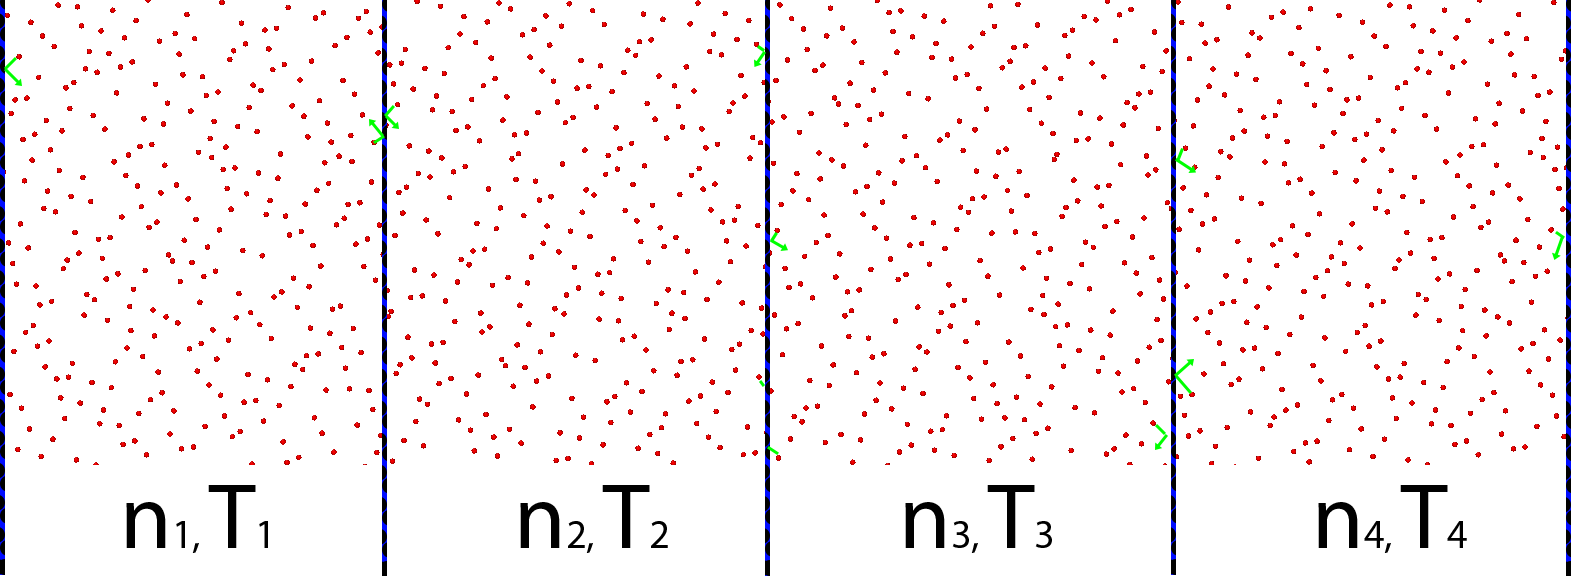
\includegraphics[width=0.8\linewidth]{equilibration.png}
	\caption{Configuration of MD simulation during equilibration phase.}
	\label{MDequil}
\end{figure}

Once equilibrated, we throw away the velocities of each particle, and draw new velocities for every particle in cell $x_i$ from the velocity distribution at $x_i$, $f_k(x_i,\mathbf{v},t)$. Because this distribution is very discrete in the kinetic formulation, we linearly interpolate it before sampling. This method is able to accurately capture in MD at least the first four moments of the $f_k$ distribution with sufficient particles. Once this is done, the particles have correlated spatially and are distributed according to the correct velocity distribution. This is considered the ``initial condition'' for an MD simulation.

The MD simulation is run for a period of time, and the positions and velocities are recorded for use in compression. Each $f_k$ is approximated by $E[g_k]$. That is, we record the number of ions of species $k$ that have $x$ positions in $[x,x+\Delta x]$ with velocities in $[\mathbf{v},v+\Delta \mathbf{v}]$ at each timestep. The average of this is $E[g_k]$, and $E[g]=\sum_k E[g_k]$. The moments of $E[g_k]$ can be computed and used to define the $f_{kl}^{eq}$ Maxwellian distributions.

Using the time series for $E[g_k]$, we can compute $\frac{\partial E[g_k]}{\partial t}$ using a second order centered difference scheme averaged over many timesteps. The gradient $\mathbf{F}_k=\nabla_\mathbf{r}(f_k\log(f))$ can be computed by using a centered difference spatial derivative on $E[g_k]\log(E[g])$. In the single species case, we have now computed every quantity needed to calculate $\tau(\mathbf{r}_n)$ from (\ref{eq:dHdt}).

In the multispecies case, we now use the $E[g_k]$ to compute $\rho_k$, and solve the Poisson equation using a linear solve with the standard centered difference Poisson operator to compute each $\mathbf{E}_k$. The densities and bulk velocities $n_k$ and $\mathbf{u}_k$ can be computed from the moments of $E[g_k]$. Finally, the expected interparticle forces $\mathbf{f}_{ij}$ and kinetic energies $K_k$ are computed each timestep already, and so can be recorded. The equilibrium kinetic energies $K_{kl}^{eq}$ are again determined by the equilibrium distributions.

From this, we can now compute every cross-species $\tau_{kl}$ using (\ref{eq:taukl}), and we then use these in (\ref{eq:taukk}) to compute the intraspecies $\tau_{kk}$. Note that the $(\Delta r)^d$ is actually equal to $(\Delta x)L_y$ because we are averaging out the $y$ dimension. This is the case for every spatial integral.

The simulation is run for a period of time. Positions and velocities are recorded, and used to compute the expected values needed to compute $\tau_{kl}(x)$ and $f_k(x,\mathbf{v},t)$. Once the statistics on these quantities are sufficiently accurate, the MD simulation ends and the $\tau_{kl}(x)$ and $f_k(x,\mathbf{v},t)$ are used to initialize another BGK simulation period.

We continue to compute $\frac{d H^{BGK}}{dt}$ during our BGK simulation. Once this changes sufficiently from its initial value, we consider the $\tau_{kl}$ values ``stale'' and reinitialize an MD simulation to update them.

%----------------------------------------------------------------------------------------
\subsection{Parametrization}
%----------------------------------------------------------------------------------------

We wish to study plasmas that meet certain collisionality criteria, such that a kinetic perspective is warranted. For this reason, it is useful to rewrite the governing equations in a parameterized, dimensionless form. We first choose our length scale as the ion-circle radius $a$. We then define a dimensionless coupling parameter $\Gamma$ that describes the ratio of the potential energy to the kinetic energy of the system, a dimensionless screening parameter $\kappa$ that describes the extent to which the background electrons screen the electrostatic field of the ions, and a plasma frequency $\omega_p$ that defines an important timescale. These parameters are defined as
\begin{align}
a^2 &= \frac{1}{\pi n} \\
\Gamma &= \frac{Z^2e^2}{4\pi\epsilon_0aT} \\
\kappa &= \frac{a}{\lambda}\\
\omega_p^2 &= \frac{Z^2e^2n}{2\epsilon_0am}.
\end{align}

Since the properties of the system vary in space and time, it is convenient to define reference parameters $a_0$, $\omega_0$, and $m_0$. We define $a_0$ based on the average density $n_{avg}$, so that $\pi a_0^2n_{avg}=1$. Therefore, on average there is a distance of $a_0$ between neighboring ions. It is also helpful to define $\omega_0$ with $Z=1$ for notational simplicity. The reference mass $m_0$ may be arbitrary. One choice is to use the mass of the lightest particle species of interest. The fundamental scaled variables, denoted by the tilde, are defined as:
\begin{align*}
\text{Length:}&			&\tilde{x} &= \frac{x}{a_0} 	\\
\text{Time:}&			&\tilde{t} &= \omega_0 t 	\\
\text{Mass:}&			&\tilde{m} &= \frac{m}{m_0}.
\end{align*}
From these we can construct the scaled versions of all derived quantities:
\begin{align*}
\text{Velocity:}&			&	\tilde{\mathbf{v}} 	 &= \frac{\mathbf{v}}{a_0\omega_0} 				\\
\text{Force:}&				&	\tilde{F} 	 &= \frac{F}{a_0\omega_0^2m_0}			\\
\text{Energy:}&				&	\tilde{U} 	 &= \frac{U}{a_0^2\omega_0^2m_0} 		\\
\text{Distribution:}& 		&	\tilde{f} 	 &= \frac{f}{a_0^4\omega_0^2}			\\
\text{Electric Potential:}& &	\tilde{\phi} &= \frac{\phi e}{a_0^2\omega_0^2m_0}	\\
\text{Density:}&			&	\tilde{n}	 &= na_0^2								\\
\text{Temperature:}&        &	\tilde{T}	 &= \frac{T}{a_0^2\omega_0^2m_0}.
\end{align*}
The coupling parameter and plasma frequency in any given region of the domain can then be written in terms of the dimensionless parameters:
\begin{align}
\Gamma&=\frac{Z^2\sqrt{\pi\tilde{n}}}{2\tilde{T}}\\
\omega_p^2&=\frac{Z^2(\pi\tilde{n})^{3/2}}{\tilde{m}}\omega_0^2.
\end{align}
In the weakly to moderately coupled regime that we are studying, $\Gamma$ should be approximately $O(0.1-1)$. If the system is too weakly collisional, it will behave as an ideal gas, where collisions are not significant. If the system is very strongly collisional, then collisional effects dominate and the system is best be modeled with hydrodynamic equations. We wish to select a regime in which the kinetic scale is the most relevant. This formulation also places a constraint on the average dimensionless density of the system such that $\tilde{n}_{avg}=\frac{1}{\pi}$ so that $a_0$ corresponds to the average ion-circle radius in the domain. For our computations, we use a screening parameter $\kappa=1$.

The dimensionless kinetic equations are nearly identical to the dimensional version, with the exception of the Poisson equation. The dimensionless distribution function, $\tilde{f}_k$, evolves according to
\begin{align*}
&\frac{\partial \tilde{f}_k}{\partial \tilde{t}}+\tilde{v}_{\tilde{x}}\frac{\partial \tilde{f}_k}{\partial \tilde{x}}+\frac{\tilde{Z}_k}{\tilde{m}_k}\tilde{E}(\tilde{x})\frac{\partial \tilde{f}_k}{\partial \tilde{v}_{\tilde{x}}}=\sum_l\frac{\tilde{f}_{kl}^{eq}-\tilde{f}_k}{\tilde{\tau}_{kl}}\\
&\tilde{E}(x) = -\frac{1}{2}\int\tilde{x}'\tilde{\rho}(\tilde{x}-\tilde{x}')\int\frac{e^{-\kappa|\tilde{\mathbf{r}}'|}}{|\tilde{\mathbf{r}}'|^2}\left(\frac{1}{|\tilde{\mathbf{r'}}|}-\kappa\right)\,d\tilde{y}'\,d\tilde{x}'
\end{align*}
where $\tilde{\rho} = \sum_{l}Z_l\tilde{n}_l$. The moments of the distribution function become
\begin{align*}
\tilde{n}_k &= \int\tilde{f}_k\,d\tilde{\mathbf{v}} \\
\tilde{\mathbf{u}}_k &= \frac{1}{\tilde{n}_k}\int\tilde{\mathbf{v}}\tilde{f}_k\,d\tilde{\mathbf{v}} \\
\tilde{T}_k &= \frac{\tilde{m}_k}{2\tilde{n}_k}\int\left|\tilde{\mathbf{v}}-\tilde{\mathbf{u}}_k\right|^2\tilde{f}_k\,d\tilde{\mathbf{v}}.
\end{align*}
As with the kinetic equations, the dimensionless MD equations are essentially unchanged. Only the potential term differs. The velocity Verlet algorithm becomes:
\begin{align*}
\tilde{\mathbf{v}}_i\left(\tilde{t}+\frac{\Delta\tilde{t}}{2}\right) &= \tilde{\mathbf{v}}_i(\tilde{t}) + \frac{\Delta\tilde{t}}{2}\frac{\tilde{\mathbf{F}}_i(\tilde{t})}{\tilde{m}_i} \\
\tilde{\mathbf{r}}_i(\tilde{t}+\Delta\tilde{t}) &= \tilde{\mathbf{r}}_i(\tilde{t}) + \Delta\tilde{t}\:\tilde{\mathbf{v}}_i\left(\tilde{t}+\frac{\Delta\tilde{t}}{2}\right) \\
\tilde{\mathbf{v}}_i(\tilde{t}+\Delta\tilde{t}) &= \tilde{\mathbf{v}}_i\left(\tilde{t}+\frac{\Delta\tilde{t}}{2}\right) + \frac{\Delta\tilde{t}}{2}\frac{\tilde{\mathbf{F}}_i(\tilde{t}+\Delta\tilde{t})}{\tilde{m}_i}.
\end{align*}
During the equilibration phase, the Langevin velocity Verlet algorithm becomes
\begin{align*}
\tilde{\mathbf{v}}_i\left(\tilde{t}+\frac{\Delta\tilde{t}}{2}\right) &= \tilde{\mathbf{v}}_i\left(\tilde{t}\right) + \frac{\Delta\tilde{t}}{2}\frac{\tilde{\mathbf{F}}_i\left(\tilde{t}\right)}{\tilde{m}_i} - \frac{\tilde{\gamma}_i\Delta\tilde{t}}{2}\left(\tilde{\mathbf{v}_i}\left(\tilde{t}\right)\right) + \sqrt{\frac{\tilde{\gamma}_i\Delta\tilde{t}\:\tilde{T}}{\tilde{m}_i}}\eta \\
\tilde{\mathbf{r}}_i\left(\tilde{t}+\Delta\tilde{t}\right) &= \tilde{\mathbf{r}}_i\left(\tilde{t}\right) + \Delta\tilde{t}\:\tilde{\mathbf{v}}_i\left(\tilde{t}+\frac{\Delta\tilde{t}}{2}\right) \\
\tilde{\mathbf{v}}_i\left(\tilde{t}+\Delta\tilde{t}\right) &= \left(1+\frac{\tilde{\gamma}_i\Delta\tilde{t}}{2}\right)^{-1} \left(\tilde{\mathbf{v}}_i\left(\tilde{t}+\frac{\Delta\tilde{t}}{2}\right) + \frac{\Delta\tilde{t}}{2}\frac{\tilde{\mathbf{F}}_i\left(\tilde{t}+\Delta\tilde{t}\right)}{\tilde{m}_i} + \sqrt{\frac{\tilde{\gamma}_i\Delta\tilde{t}\tilde{T}}{\tilde{m}_i}}\eta\right).
\end{align*}
The Yukawa potential and force equations become
\begin{align*}
\tilde{V}_{ij}&=\frac{\tilde{Z}_i\tilde{Z}_j}{2|\tilde{\mathbf{r}}_i-\tilde{\mathbf{r}}_j|}e^{-\kappa|\tilde{\mathbf{r}}_i-\tilde{\mathbf{r}}_j|}\\
\tilde{F}_{ij}&=\tilde{V}_{ij}\left(\frac{1}{|\tilde{\mathbf{r}}_i-\tilde{\mathbf{r}}_j|}+\kappa\right)\frac{\tilde{\mathbf{r}}_i-\tilde{\mathbf{r}}_j}{|\tilde{\mathbf{r}}_i-\tilde{\mathbf{r}}_j|}.
\end{align*}
The dimensionless energies and moments are
\begin{align*}
\tilde{\text{PE}} 	&= \frac{1}{2}\sum_{i\neq j}\tilde{V}_{ij} \\
\tilde{\text{KE}} 	&= \frac{1}{2}\sum_{i}\tilde{m}_i|\tilde{\mathbf{v}}_i|^2 \\
\tilde{\text{TE}} 	&= \tilde{\text{PE}} + \tilde{\text{KE}} \\
\tilde{n}_k			&= \frac{N_k}{\tilde{A}} \\
\tilde{\mathbf{u}}_k			&= \frac{1}{N_k}\sum_{i\in S_k}\tilde{\mathbf{v}}_i \\
\tilde{T}_k			&= \frac{1}{N_{DoF}}\sum_{i\in S_k}\tilde{m}_k\left|\tilde{\mathbf{v}}_i-\tilde{\mathbf{u}}_k\right|^2.
\end{align*}
The moments are time-averaged quantities, since thermal noise affects each of them to some degree.

\newpage
\bibliography{MultiScale}
\bibliographystyle{plain}
\end{document}